\chapter{Teoría de la computabilidad}

\section{Computabilidad: Enfoque inductivo}

En esta sección abordaremos el enfoque inductivo de la computabilidad. Este se caracteriza por la construcción de lo computable por medio de ciertas funciones básicas y operaciones que permiten combinarlas. Frente al enfoque mecánico, el cual concibe un algoritmo como una secuencia de pasos ejecutados en el tiempo, este enfoque nos describe lo computable de una manera estructural: un algoritmo deja de ser una lista finita de instrucciones y, en cambio, se vuelve una combinación de otros algoritmos más simples. Este enfoque tiene como ventaja el poder justificar la computabilidad de una función por medio de la verificación de propiedades de cerradura; en lugar de exhibir una lista de pasos explícitos para cada función, solamente es necesario verificar que la función puede derivarse de otras que ya conozcamos como computables y que se obtengan mediante operaciones admisibles.

\subsection{Funciones primitivo-recursivas}

El primer tipo de funciones que abordaremos son las \emph{funciones primitivo-recursivas}. El interés sobre este tipo de funciones es, por una parte, debido a que abarcan la mayoría de los objetos computables que podemos encontrarnos en la práctica; y por otra, a que son la mayoría de objetos que construiremos para estudiar la computabilidad.

La característica principal de las funciones primitivo-recursivas es que se obtienen de funciones básicas mediante composición y recursión primitiva. La composición corresponde a la idea de poder utilizar diferentes algoritmos como subrutinas auxiliares que permitan ejecutar un algoritmo más complejo. La recursión, por su parte, puede interpretarse como un ciclo \emph{for}: el número de iteraciones queda determinado de antemano por los argumentos de la función, de modo que no solo tenemos la certeza de que el proceso ejecutará un número finito de pasos, sino de cuántos de ellos exactamente. Estos conceptos se definen formalmente de la siguiente manera.

\begin{definition}[Funciones primitivo-recursivas]
	\label{def: funciones_primitivas}
	Sea $n\in\omega^{+}$. Una función $f:\omega^{n}\to\omega$ se denomina \emph{primitivo-recursiva} si satisface alguna de las siguientes condiciones:
	\begin{enumerate}
		\item (Funciones básicas) La función $f$ es una de las siguientes funciones:
		\begin{itemize}
			\item La función \emph{cero}: $\CERO:\omega^{n}\to\omega$ tal que para cada $x\in\omega^{n}$, $\CERO(x) = 0$.
			\item Si $n = 1$, la función \emph{sucesor}: $\SUCESOR:\omega\to\omega$ tal que para cada $x\in\omega$, $\SUCESOR(x) = x + 1$.
			\item Para algún $k\in\omega^{+}$ con $k\leq n$, la función \emph{proyección}: $\PROYECCION{n}{k}:\omega^{n}\to\omega$ tal que para cada $x_{1},\dotsc, x_{n}\in\omega$, $\PROYECCION{n}{k}\pa{x_{1},\dotsc, x_{n}} = x_{k}$.
		\end{itemize}
		\item (Composición) Para algún $m\in\omega^{+}$ existen funciones primitivo-recursivas $g_{1},\dotsc, g_{m}:\omega^{n}\to\omega$ y $h:\omega^{m}\to\omega$ tales que para cada $x\in\omega^{n}$, $f(x) = h\pa{g_{1}(x),\dotsc, g_{m}(x)}$.
		\item (Recursión) Si $n > 1$ y existen funciones primitivo-recursivas $g:\omega^{n - 1}\to\omega$ y $h:\omega^{n + 1}\to\omega$ tales que para cada $x\in\omega^{n - 1}$ y cada $y\in\omega$ se satisface que:
		\[
			\begin{NiceArray}{c}
				f(x, 0) = g(x)\\
				f(x, y + 1) = h(x, y, f\pa*{x, y})
			\end{NiceArray}
		\]
	\end{enumerate}
	
	Para cada $n\in\omega^{+}$, denotamos por $\PRIMITIVO[n]$ al conjunto de todas las funciones primitivo-recursivas de aridad $n$. Definimos al conjunto de funciones primitivo-recursivas como $\PRIMITIVO\coloneqq\bigcup_{n\in\omega^{+}}\PRIMITIVO[n]$.
\end{definition}

Ejemplo de cómo es que estas funciones modelan una parte de la computabilidad es el siguiente teorema.

\begin{theorem}
	La suma, producto, exponenciación y las funciones constantes son funciones primitivo-recursivas.
\end{theorem}

Antes de ir a la demostración formal, veamos cómo es que podemos reescribir a estas funciones. Para el caso de la suma, notemos que si $\mathrm{Suma}\left(x, y\right) = x + y$, entonces:
\[
	\mathrm{Suma}\pa*{x, y + 1} = x + (y + 1) = (x + y) + 1 = \mathrm{Suma}\pa*{x, y} + 1
\]
por lo que la suma puede escribirse de manera recursiva sobre el segundo argumento. Notemos que para que la recursión esté bien definida necesitamos tener un caso base. En este caso tendríamos que $\mathrm{Suma}\left(x, 0\right) = x + 0 = x$.

Similarmente para el caso del producto, si $\mathrm{Prod}\pa*{x, y} = xy$, entonces:
\[
\mathrm{Prod}\pa*{x, y + 1} = x(y + 1) = xy + x = \mathrm{Prod}\pa*{x, y} + x
\]
con el caso base $\mathrm{Prod}\pa*{x, 0} = x\cdot 0 = 0$.

Ahora para la exponenciación, si $\mathrm{Exp}\pa*{x, y} = x^{y}$, entonces:
\[
\mathrm{Exp}\pa*{x, y + 1} = x^{y + 1} = x^{y}x = \mathrm{Exp}\pa*{x, y}x
\]
con el caso base $\mathrm{Exp}\pa*{x, 0} = x^{0} = 1$.

Con esto vemos que estas operaciones pueden calcularse de manera recursiva, lo cual nos es de ayuda para poder utilizar recursión primitiva y así ver que estas funciones son primitivo-recursivas.

\begin{proof}
	Para el caso de la suma definamos la función $f:\omega^{2}\to\omega$ como:
	\[
		\begin{NiceArray}{c}
			f(x, 0) =\PROYECCION{1}{1}(x)\\
			f(x, y + 1) =\SUCESOR\pa{\PROYECCION{3}{3}\pa{x, y,f\pa*{x, y}}}
		\end{NiceArray}
	\]
	
	Puesto que $\PROYECCION{1}{1}$, $\SUCESOR$ y $\PROYECCION{3}{3}$ son funciones primitivo-recursivas, se tiene que $f$ es primitivo-recursiva. Mostremos entonces que para cada $x, y\in\omega$ se satisface que $f\pa*{x, y} = x + y$. Mostremos por inducción sobre $y$. 
	\begin{itemize}
		\item (Base) Se tiene que para $y = 0$ se sigue que $f(x, 0) = \PROYECCION{1}{1}(x) = x = x + y$. 
		\item (Paso inductivo) Sea $y\in\omega$ tal que $f\pa*{x, y} = x + y$. Entonces mostremos que $f(x, y + 1) = x + (y + 1)$. Por la definición de $f$ se tiene lo siguiente:
		\[
			f(x, y + 1) =\SUCESOR\pa{\PROYECCION{3}{3}\pa{x, y,f\pa*{x, y}}} = \SUCESOR\pa{f\pa*{x, y}} = f\pa*{x, y} + 1 = (x + y) + 1 = x + (y + 1)
		\]
		Probando así la proposición.
	\end{itemize}
	
	
	Ahora, para el caso del producto definamos la función auxiliar $g: \omega^3\to\omega$ para cada $x, y, z\in\omega$ como:
	\[
		g(x, y, z) = \PROYECCION{3}{3}\pa*{x, y, z} + \PROYECCION{3}{1}\pa*{x, y, z}
	\]
	la cual es primitivo-recursiva debido a que $\PROYECCION{3}{1}$, $\PROYECCION{3}{3}$ y la suma lo son. Ahora, el producto puede describirse como la función $f:\omega^{2}\to\omega$ tal que:
	\[
		\begin{NiceArray}{c}
			f(x, 0) =\CERO(x)\\
			f(x, y + 1) = g\pa*{x, y, f\pa*{x, y}}
		\end{NiceArray}
	\]
	Puesto que $\operatorname{Z}$ y $g$ son funciones primitivo-recursivas, se tiene que $f$ es primitivo-recursiva. Mostremos entonces que para cada $x, y\in\omega$ se satisface que $f\pa*{x, y} = xy$. Mostremos por inducción sobre $y$.
	\begin{itemize}
		\item (Base) Se tiene que para $y = 0$ se sigue que $f(x, 0) = \CERO(x) = 0 = xy$. 
		\item (Paso inductivo) Sea $y\in\omega$ tal que $f\pa*{x, y} = xy$. Entonces mostremos que $f(x, y + 1) = x(y + 1)$. Por la definición de $f$ se tiene lo siguiente:
		\begin{align*}
			f(x, y + 1) &= g(x, y, f\pa*{x, y}) \\
			&=\PROYECCION{3}{3}\pa{x, y, f\pa*{x, y}} +\PROYECCION{3}{1}\pa*{x, y}\\
			&= f\pa*{x, y} +\PROYECCION{2}{1}\pa*{x, y} \\
			&= f\pa*{x, y} + x \\
			&= xy + x\\
			&= x\pa*{y + 1}
		\end{align*}
		Probando así la proposición.
	\end{itemize}
	
	Para el caso de la exponenciación definamos a la función auxiliar $h: \omega^3\to\omega$ tal que:
	\[
		h(x, y, z) = \PROYECCION{3}{3}(x, y, z)\PROYECCION{3}{1}(x, y, z)
	\]
	la cual podemos asegurar que es primitivo-recursiva ya que $\PROYECCION{3}{1}$, $\PROYECCION{3}{3}$ y el producto lo son. Por lo tanto, la exponenciación puede describirse mediante la función $f:\omega^{2}\to\omega$ tal que:
	\[
	\begin{NiceArray}{c}
		f(x, 0) =\SUCESOR\pa{\CERO(x)}\\
		f(x, y + 1) = h\pa*{x, y, f\pa*{x, y}}
	\end{NiceArray}
	\]
	Puesto que $\SUCESOR$, $\CERO$ y $h$ son funciones primitivo-recursivas, se tiene que $f$ es primitivo-recursiva. Mostremos entonces que para cada $x, y\in\omega^{+}$ se satisface que $f\pa*{x, y} = x^{y}$. Prosigamos por inducción sobre $y$. 
	\begin{itemize}
		\item (Base) Para $y = 0$ se sigue que $f(x, 0) = \SUCESOR\pa{\CERO(x)} = 1 = x^{y}$. 
		\item (Paso inductivo) Sea $y\in\omega$ tal que $f(x, y) = x^{y}$. Entonces mostremos que $f(x, y + 1) = x^{y + 1}$. Por la definición de $f$ se tiene lo siguiente:
		\begin{align*}
			f(x, y + 1) &= h\pa*{x, y, f\pa*{x, y}}\\
			&=\PROYECCION{3}{3}\pa{x, y, f\pa*{x, y}}\PROYECCION{3}{1}\pa*{x, y, f\pa*{x, y}}\\
			&= f\pa*{x, y}x \\
			&= x^{y}x\\
			&= x^{y + 1}
		\end{align*}
		Probando así la proposición.
	\end{itemize}
	
	Para cada $m\in\omega$ y cada $n\in\omega^{+}$ denotemos por $f_{m}^{n}:\omega^{n}\to\omega$ a la función constante $m$, es decir, tal que para cada $x\in\omega^{n}$ se satisface que $f_{m}^{n}\left(x\right) = m$. Mostremos por inducción sobre la constante $m$ que $f_{m}^{n}$ es primitivo-recursiva.
	\begin{itemize}
		\item (Base) Sea $n\in\omega^{+}$. Para la función $f_{0}^{n}$ claramente que tiene que $f_{0}^{n} =\CERO\circ\PROYECCION{n}{1}$. Puesto que $f_{0}^{n}$ es composición de funciones básicas, entonces es primitivo-recursiva.
		\item (Paso inductivo) Sean $n\in\omega^{+}$ y $m\in\omega$ tales que $f_{m}^{n}$ es primitivo-recursiva. Notemos que $f_{m + 1}^{n} = \SUCESOR\circ f_{m}^{n}$. Puesto que $\SUCESOR$ es una función básica y $f_{m}^{n}$ es primitivo-recursiva, entonces $f_{m + 1}^{n}$ es primitivo-recursiva.
	\end{itemize}
	
	Por lo tanto, para cada $n\in\omega^{+}$ y cada $m\in\omega$ se tiene que $f_{m}^{n}$ es primitivo-recursiva.
\end{proof}

De la demostración anterior puede apreciarse que usar recursión es equivalente al uso de un \emph{for} algorítmicamente hablando. Para el caso de la suma se tendría que $x + y$ comprendería ejecutar un algoritmo que devuelve el valor $x$ si $y = 0$ y, en caso contrario, suma uno al valor $x$ un número $y$ de veces.

\begin{algorithm}[h!]
	\caption{Suma}
	\begin{algorithmic}
		\Require $x$, $y$
		\Ensure $x + y$
		\For{$n = 0,\dotsc, y - 1$}
		\State $x \gets x + 1$
		\EndFor
		\State \Return $x$
	\end{algorithmic}
\end{algorithm}

En cuanto al producto $xy$ se trataría de un algoritmo el cual utiliza un ciclo \emph{for} que va sumando repetidamente el valor $x$ un número $y$ de veces. De manera similar para el caso de la exponenciación, el cual utilizaría un ciclo *for* para ir multiplicando el valor $x$ un número $y$ de veces.

\begin{algorithm}[h!]
	\caption{Producto}
	\begin{algorithmic}
		\Require $x$, $y$
		\Ensure $xy$
		\State $z\gets 0$
		\For{$n = 0,\dotsc, y - 1$}
		\State $z \gets \text{Suma}(z, x)$
		\EndFor
		\State \Return $z$
	\end{algorithmic}
\end{algorithm}

\begin{algorithm}[h!]
	\caption{Exponenciación}
	\begin{algorithmic}
		\Require $x$, $y$
		\Ensure $x^{y}$
		\State $z\gets 1$
		\For{$n = 0,\dotsc, y - 1$}
		\State $z \gets \text{Producto}(z, x)$
		\EndFor
		\State \Return $z$
	\end{algorithmic}
\end{algorithm}

Para poder demostrar que otras funciones comunes (y particularmente las unarias) son funciones primitivo-recursivas debemos demostrar que es posible debilitar la recursión primitiva. Observemos que en la definición \ref{def: funciones_primitivas} se nos permite utilizar recursión primitiva únicamente cuando la función a calcular tiene al menos dos argumentos. Sin embargo, existen funciones que pueden calcularse recursivamente mediante un solo argumento (como el factorial). Por lo tanto, es necesario demostrar que utilizar este tipo de recursión más débil también genera funciones primitivo-recursivas.

\begin{theorem}[Recursión simple]
	Sean $a\in\omega$ y $g:\omega^{2}\to\omega$ primitivo-recursiva. Entonces la función $f:\omega\to\omega$ definida como sigue, para cada $x\in\omega$, es primitivo-recursiva:
	\[
		\begin{NiceArray}{c}
			f\pa*{0} = a\\
			f\pa*{x + 1} = g\pa*{x, f\pa*{x}}
		\end{NiceArray}
	\]
\end{theorem}

\begin{proof}
	Consideremos primero a las funciones auxiliares $h_0:\omega^3\to\omega$ tal que $h_0 = g(\PROYECCION{3}{2},\PROYECCION{3}{3})$ y $h:\omega^{2}\to\omega$ definida como sigue para cada $x, y\in\omega$:
	
	\[
	\begin{NiceArray}{c}
		h\pa*{x, 0} = f^{1}_{a}\pa*{x}\\
		h\pa*{x, y + 1} = h_0\pa*{x, y, h\pa*{x, y}}
	\end{NiceArray}
	\]
	
	Notemos que las funciones $h_0$ y $h$ son primitivo-recursivas puesto que $g$ y las funciones proyección son primitivo-recursivas. Afirmamos que $h$ es una extensión de $f$ donde su primer argumento no afecta a la recursión, de modo que $f = h\pa*{\CERO, \PROYECCION{1}{1}}$. Mostremos tal afirmación por inducción:
	\begin{itemize}
		\item (Base) Se tiene que $h\pa*{\CERO\pa*{0},\PROYECCION{1}{1}\pa*{0}} = h\pa*{0, 0} = f_{a}^{1}\pa*{0} = a = f\pa*{0}$.
		\item (Paso inductivo) Sea $x\in\omega$ tal que $f\pa*{x} = h\pa*{\CERO\pa*{x},\PROYECCION{1}{1}\pa*{x}} = h\pa*{0, x}$, entonces se tiene que:
		\begin{align*}
			h\pa*{\CERO\pa*{x + 1},\PROYECCION{1}{1}\pa*{x + 1}} &= h\pa*{0, x + 1}\\
			&= h_{0}\pa*{0, x, h\pa*{0, x}}
			&= g\pa*{\PROYECCION{3}{2}\pa*{0, x, h\pa*{0, x}}, \PROYECCION{3}{3}\pa*{0, x, h\pa*{0, x}}}\\
			&= g\pa*{x, h\pa*{0, x}}\\
			&= g\pa*{x, f\pa*{x}}\\
			&= f\pa*{x + 1}
		\end{align*}
	\end{itemize}
	Por lo tanto, se cumple que $f = h\pa*{\CERO,\PROYECCION{1}{1}}$, la cual es primitivo-recursiva ya que $h$ es primitivo-recursiva.
\end{proof}

Con este teorema podemos entonces demostrar que las funciones factorial, predecesor y resta son primitivo-recursivas.

\begin{theorem}
	Las siguientes funciones son primitivo-recursivas.
	\begin{enumerate}
		\item El factorial, es decir, la función $f:\omega\to\omega$ tal que para cada $x\in\omega$:
		\[
			f(x) =
			\begin{cases}
				1, & x = 0\\
				1\cdot2\cdot\dotsc\cdot x, & x > 0
			\end{cases}
		\]
		\item La función predecesor, es decir, la función $f:\omega\to\omega$ tal que para cada $x\in\omega$:
		\[
			f(x) =
			\begin{cases}
				0, & x = 0\\
				x - 1, & x > 0
			\end{cases}
		\]
		\item La función resta en $\omega$, es decir, la función $f:\omega^{2}\to\omega$ tal que para cada $x, y\in\omega$:
		\[
			f\pa*{x, y} =
			\begin{cases}
				0, & x\leq y\\
				x - y, & x > y
			\end{cases}
		\]
	\end{enumerate}
\end{theorem}

\begin{proof}
	Para el factorial notemos que tal función se puede definir de la siguiente manera recursiva:
	\[
		\begin{NiceArray}{c}
			f\pa*{0} = 1\\
			f\pa*{x + 1} = \pa*{x + 1}\cdot f\pa*{x}
		\end{NiceArray}
	\]
	la cual es primitivo-recursiva por los teoremas anteriores.
	
	En el caso de la función predecesor, se puede definir recursivamente como sigue:
	\[
		\begin{NiceArray}{c}
			f\pa*{0} = 0\\
			f\pa*{x + 1} = \PROYECCION{2}{1}\pa*{x, f\pa*{x}}
		\end{NiceArray}
	\]
	la cual es primitivo-recursiva por los teoremas anteriores igualmente. Denotemos a la función predecesor como $\mathrm{Pred}\pa*{x}$. 
	
	Para el caso de la resta, esta se puede definir recursivamente como sigue:
	\[
		\begin{NiceArray}{c}
			f\pa*{x, 0} =\PROYECCION{1}{1}\pa*{x}\\
			f\pa*{x, y + 1} = \mathrm{Pred}\pa*{\PROYECCION{3}{3}\pa*{x, y, f\pa*{x, y}}}
		\end{NiceArray}
	\]
	Mostremos en este caso que realmente se trata de la resta restringida a $\omega$ por inducción sobre el segundo argumento. Para ello, dividamos en dos casos: cuando $y\leq x$ y cuando $y > x$.
	
	Supongamos que $y\leq x\in\omega$ y mostremos por inducción sobre $y$ que $f\pa*{x, y} = x - y$.
	\begin{itemize}
		\item (Base) Directamente se tiene que $f\pa*{x, 0} =\PROYECCION{1}{1}\pa*{x} = x = x - 0 = x - y$.
		\item (Paso inductivo) Sea $y < x$ para el cual $f\pa*{x, y} = x - y$ y mostremos que $f\pa*{x, y + 1} = x -\pa*{y + 1}$.
		\begin{align*}
			f\pa*{x, y + 1} &= \mathrm{Pred}\pa*{\PROYECCION{3}{2}\pa*{x, y, f\pa*{x, y}}}\\
			&= \mathrm{Pred}\pa*{f\pa*{x, y}} \\
			&= f\pa*{x, y} - 1 \\
			&= \pa*{x - y} - 1 \\
			&= x -\pa*{y + 1}
		\end{align*}
		Notemos que en este caso, como $y < x$, entonces $f\pa*{x, y} = x - y > 0$, por lo que en efecto $\mathrm{Pred}\pa*{f\pa*{x, y}} = f\pa*{x, y} - 1$.
	\end{itemize}
	
	Ahora, para el caso cuando $y > x$, notemos que existe $z\in\omega$ para el cual $y = x + 1 + z$. Por lo tanto, mostremos por inducción sobre $z$ que $f\pa*{x, y} = 0$.
	\begin{itemize}
		\item (Base) Notemos directamente que $f\pa*{x, x + 1} =\mathrm{Pred}\pa*{f\pa*{x, x}} =\mathrm{Pred}\pa*{0} = 0$.
		\item (Paso inductivo) Sea $z\in\omega$ para el cual se satisface que $f\pa*{x, x + 1 + z} = 0$, entonces mostremos que $f\pa*{x, x + 1 + \pa*{z + 1}} = 0$.
		\begin{align*}
			f\pa*{x, x + 1 + \pa*{z + 1}}
			&= f\pa*{x, \pa*{x + 1 + z} + 1} \\
			&= \mathrm{Pred}\pa*{f\pa*{x, x + 1 + z}} \\
			&=\mathrm{Pred}\pa*{0} = 0
		\end{align*}
	\end{itemize}
	Por lo que, en efecto, se concluye que $f$ es la función resta restringida a $\omega$.
\end{proof}

Podemos extender la definición de primitivo-recursión a subconjuntos y relaciones de números naturales. Esta extensión es fundamental puesto que saber si podemos computar un conjunto es lo que nos permite determinar qué problemas pueden o no ser resueltos por medio de algoritmos. Un conjunto se dice \emph{primitivo-recursivo} si podemos determinar si un elemento pertenece a él por medio de una función primitivo-recursiva; lo cual se traduce en que su función característica es primitivo-recursiva. Más aún, esto se puede extender a propiedades. Una propiedad se denomina primitivo-recursiva si podemos \emph{decidir} si un elemento la satisface o no mediante una función primitivo-recursiva. Notemos que cualquier propiedad sobre los naturales puede ser traducida al conjunto que define, y si este conjunto es primitivo-recursivo, entonces se tiene que siempre podemos determinar si cualquier elemento la satisface.

\begin{definition}[Conjuntos primitivos recursivos]
	Sea $A\subseteq\omega^{n}$ para algún $n\in\omega^{+}$. El conjunto $A$ se dice ser \emph{primitivo-recursivo} si su función característica $\CARACTERISTICA{A}:\omega^{n}\to\omega^{+}$ es primitivo-recursiva.
\end{definition}

Ejemplos de conjuntos que son primitivos recursivos están descritos en el siguiente teorema.

\begin{theorem}
	Los conjuntos $>, <, =\subseteq\omega^{2}$, $\set{0}$ y $\omega^{+}$ son primitivos recursivos.
\end{theorem}

\begin{proof}
	Notemos que $\CARACTERISTICA{\set{0}}(x) = 1 - x$ para cada $x\in\omega$, puesto que cuando $x = 0$, se tiene que $1 - x = 1$; y cuando $x > 0$, entonces $1 - x = 0$ por definición de resta restringida. Puesto que la resta es primitivo-recursiva, se sigue que $\CARACTERISTICA{\set{0}}$ es primitivo-recursiva.
	
	Puesto que $\CARACTERISTICA{\omega^{+}}(x) = 1 -\CARACTERISTICA{\set{0}}(x)$ para cada $x\in\omega$ y $\CARACTERISTICA{\set{0}}$ es primitivo-recursiva, se sigue que $\CARACTERISTICA{\omega^{+}}$ es primitivo-recursiva.
	
	Finalmente, puesto que $\chi_{ < }\pa*{x, y} =\CARACTERISTICA{\omega^{+}}(y - x)$, $\CARACTERISTICA{>}\pa*{x, y} =\CARACTERISTICA{\omega^{+}}(x - y)$ y $\CARACTERISTICA{=}\pa*{x, y} =\CARACTERISTICA{\set{0}}\pa{\CARACTERISTICA{<}\pa*{x, y} + \CARACTERISTICA{>}\pa*{x, y}}$ para cada $x, y\in\omega$, se concluye que $\CARACTERISTICA{<}$, $\CARACTERISTICA{>}$ y $\CARACTERISTICA{=}$ son primitivo-recursivas.
\end{proof}

\begin{theorem}
	Sean $n\in\omega^{+}$ y $A, B\subseteq\omega^{n}$. Si $A$ y $B$ son primitivo-recursivos, entonces $\omega^{n}\setminus A$, $A\cup B$ y $A\cap B$ son primitivo-recursivos.
\end{theorem}

\begin{proof}
	Se tiene que $\CARACTERISTICA{\omega^{n}\setminus A} = 1 -\CARACTERISTICA{A}$, $\CARACTERISTICA{A\cap B} =\CARACTERISTICA{A}\CARACTERISTICA{B}$ y $\CARACTERISTICA{A\cup B} =\CARACTERISTICA{A} +\CARACTERISTICA{B} -\CARACTERISTICA{A\cap B}$, y puesto que $A$ y $B$ son primitivo-recursivas, se sigue que $\omega^{n}\setminus A$, $A\cup B$ y $A\cap B$ son primitivo-recursivos.
\end{proof}

\begin{coll}
	\label{coll: prim_rec_formulas}
	Sean $n\in\omega^{+}$ y $\varphi,\psi$ fórmulas con $n$ variables libres. Si $\varphi$ y $\psi$ definen conjuntos primitivos recursivos, entonces $\neg\varphi$, $\varphi\land\psi$ y $\varphi\vee\psi$ definen conjuntos primitivos recursivos en $\omega^{n}$.
\end{coll}

Lo siguiente es demostrar que la clase de funciones primitivo-recursivas es cerrada bajo ciertas operaciones, lo que será de mucha utilidad a lo largo del capítulo.

\begin{theorem}
	Sean $n\in\omega^{+}$, y $f:\omega^{n + 1}\to\omega$ y $g:\omega^{n}\to\omega$ funciones primitivo-recursivas. Entonces:
	\begin{enumerate}
		\item la función $h:\omega^{n}\to\omega$ dada por $h(x) =\sum_{z < g(x)}f(x, z)$ para cada $x\in\omega^{n}$ es primitivo-recursiva.
		\item la función $h:\omega^{n}\to\omega$ dada por $h(x) =\prod_{z < g(x)}f(x, z)$ para cada $x\in\omega^{n}$ es primitivo-recursiva.
	\end{enumerate}
\end{theorem}

\begin{proof}
	Mostremos únicamente para el primer punto puesto que el segundo es análogo. Definamos entonces la función $p:\omega^{n + 1}\to\omega$ tal que para cada $x\in\omega^{n}$:
	\[
		\begin{NiceArray}{c}
			p(x, 0) = 0\\
			p(x, y + 1) = p\pa*{x, y} + f\pa*{x, y}
		\end{NiceArray}
	\]
	Mostremos que $p\pa*{x, y} =\sum_{z < y}f(x, z)$ para cada $x\in\omega^{n}$ y $y\in\omega^{+}$ por inducción sobre $y$. 
	\begin{itemize}
		\item (Base) Se tiene que si $y = 0$, entonces: 
		\[
			p(x, 0) = 0 =\sum_{z < 0}f(x, z) =\sum_{z < y}f(x, z)
		\]
		\item (Paso inductivo) Sea $y > 0$ tal que $p\pa*{x, y} =\sum_{z < y}f(x, z)$, entonces mostremos que se cumple para $y + 1$.
		\[
			p(x, y + 1) = p\pa*{x, y} + f\pa*{x, y} =\sum_{z < y}f(x, z) + f\pa*{x, y} =\sum_{z < y + 1}f(x, z)
		\]
		Probando así lo que se requería. Puesto que $f$ es primitivo-recursiva, se sigue que $p$ es primitivo-recursiva. De lo anterior se sigue entonces que $h(x) = p(x, g(x))$, y luego $h$ es primitivo-recursiva ya que $p$ y $g$ lo son.
	\end{itemize}
\end{proof}

\begin{notation}
	Sean $t\in\omega$, $n\in\omega^{+}$ y $R\subseteq\omega^{n + 1}$, entonces para cada $x\in\omega^{n}$ denotamos por:
	\begin{itemize}
		\item $\pa*{\exists m < t}R\pa*{x, m}$ a la expresión $\exists m\pa*{\pa*{m < t}\land\pa*{\pa*{x,  m}\in R}}$.
		\item $\pa*{\forall m < t}R\pa*{x}$ a la expresión $\forall m\pa*{\pa*{m < t}\to\pa*{\pa*{x,  m}\in R}}$.
		\item $\pa*{\exists m\leq t}R\pa*{x}$ a la expresión $\exists m\pa*{\pa*{m\leq t}\land\pa*{\pa*{x,  m}\in R}}$.
		\item $\pa*{\forall m\leq t}R\pa*{x}$ a la expresión $\forall m\pa*{\pa*{m\leq t}\to\pa*{\pa*{x,  m}\in R}}$.
	\end{itemize}
\end{notation}

\begin{coll}
	\label{coll: prim_rec_acotado}
	Sean $n\in\omega^{+}$, $R\subseteq\omega^{n + 1}$ primitivo-recursivo y $f:\omega^{n}\to\omega$ primitivo-recursiva, entonces:
	\begin{itemize}
		\item el conjunto $\set{x\in\omega^{n}:\pa*{\exists z < f\pa*{x}}R\pa*{x, z}}$ es primitivo-recursivo.
		\item el conjunto $\set{x\in\omega^{n}:\pa*{\forall z < f\pa*{x}}R\pa*{x, z}}$ es primitivo-recursivo.
	\end{itemize}
\end{coll}

Antes de demostrar este corolario es importante mencionar que este tipo de expresiones son fundamentales dentro de la Teoría de la Computabilidad, y particularmente cuando desarrollemos la teoría de la Aritmética de Segundo Orden. A estas expresiones les denominamos ''búsquedas''. Por ejemplo, para verificar que la expresión $\left(\exists z < f\left(x\right)\right)R\left(x, z\right)$ es verdadera, se puede ir comprobando con todos los valores $z = 0, 1,\dotsc, f\left(x\right) - 1$ si se satisface $\left(x, z\right)\in R$, uno por uno, buscando cuál de esos valores satisface tal pertenencia; y la expresión sería falsa si nunca encontramos tal valor. Para el caso de $\left(\forall z < f\left(x\right)\right)R\left(x, z\right)$, podemos en cambio verificar si la expresión es falsa buscando entre todos los valores $z = 0, 1,\dotsc, f\left(x\right) - 1$ si $\left(x, z\right)\notin R$; y si nunca encontramos tal contraejemplo, entonces la expresión original es verdadera.

Es importante notar que los procedimientos descritos siempre terminan, pues existe un número finito de candidatos (los valores entre $0$ y $f\left(x\right)$) que podemos verificar. No importa si en la práctica tarda demasiado verificar todos y cada uno de ellos, teóricamente siempre podemos decidir si las expresiones son verdaderas o falsas.

Ahora, para demostrar que estos conjuntos son primitivo-recursivos la idea es justamente saber cuándo las fórmulas son verdaderas. Para el caso de $\left(\exists z < f\left(x\right)\right)R\left(x, z\right)$, como mencionamos anteriormente, podemos verificar si alguno de los valores $\chi_{R}(x, 0)$, $\chi_{R}(x, 1)$,$\dotsc$, $\chi_{R}(x, f(x) - 1)$ es igual a uno; si al menos un término es igual a uno, entonces la fórmula se satisface. La forma de condensar esto en una única expresión es sumar todos los valores, pues la suma será mayor que cero si al menos un valor satisface la fórmula, y será cero si ninguno la satisface, de modo que podemos devolver uno si la suma es mayor que cero y devolvemos cero en caso contrario.

De manera similar, para la expresión $\left(\forall z < f\left(x\right)\right)R\left(x, z\right)$ debemos verificar que todos los valores $\chi_{R}(x, 0), \chi_{R}(x, 1),\dotsc, \chi_{R}(x, f(x) - 1)$ son uno para que la fórmula se satisfaga. Eso podemos lograrlo multiplicando todos los valores; si todos son uno, el producto será uno (indicando que la fórmula se satisface), y si al menos uno es cero, entonces el producto será cero (indicando que la fórmula es falsa). 

\begin{proof}
	Denotemos a los conjuntos como $S =\set{x\in\omega^{n}:\pa*{\exists z < f\pa*{x}}R\pa*{x, z}}$ y $T =\set{x\in\omega^{n}:\pa*{\forall z < f\pa*{x}}R\pa*{x, z}}$, entonces se tiene que:
	\[
		\begin{NiceArray}{c}
			\CARACTERISTICA{S}(x) =\CARACTERISTICA{\omega^{+}}\pa*{\sum\limits_{z < f(x)}\CARACTERISTICA{R}(x, z)}\\
			\CARACTERISTICA{T}(x) =\prod\limits_{z < f(x)}\CARACTERISTICA{R}(x, z)
		\end{NiceArray}
	\]
	
	Puesto que $f$ y $R$ son primitivos recursivos, se sigue que $S$ y $T$ son primitivos recursivos.
\end{proof}

Cuando hablamos de computación, una herramienta fundamental en la práctica es el control de flujo \emph{if-then-else}. Varias veces necesitamos que un programa computacional sea capaz de distinguir entre diferentes escenarios y realizar entonces acciones específicas para cada uno. Resulta relevante que esta estructura pueda ser modelada dentro de esta teoría. Notemos que una expresión \emph{if-then-else} tiene la siguiente forma:

\begin{algorithm}[h!]
	\caption{\emph{if-then-else}}
	\begin{algorithmic}
		\If{$R_{1}\pa*{x}$}
		\State \Return $g_{1}\pa*{x}$
		\ElsIf{$R_{2}\pa*{x}$}
		\State\Return $g_{2}\pa*{x}$
		\State $\vdots$
		\ElsIf{$R_{m}\pa*{x}$}
		\State\Return $g_{m}\pa*{x}$
		\Else
		\State\Return $g_{m + 1}\pa*{x}$
		\EndIf
	\end{algorithmic}
\end{algorithm}

Donde las expresiones $R_1,\dotsc, R_m$ son las condiciones (disjuntas) que nos permiten discernir entre los diferentes escenarios y las cuales se evalúan para determinar si alguna se satisface para entonces ejecutar el código descrito por $g_k$ para algún $k\leq m + 1$. Como hemos descrito anteriormente, una condición o propiedad se corresponde con el conjunto que define; por lo que las condiciones pueden verse como relaciones primitivo-recursivas disjuntas. Para el caso de los códigos de cada rama, estos pueden ser representados como funciones primitivo-recursivas (nuestra forma de modelar un algoritmo hasta ahora). Por lo tanto, una expresión \emph{if-then-else} puede modelarse dentro de este marco como una función primitivo-recursiva definida a trozos.

\begin{theorem}
	Sean $n, m\in\omega^{+}$, funciones primitivo-recursivas $g_{1},\dotsc, g_{m}, g_{m + 1}:\omega^{n}\to\omega$ y relaciones primitivo-recursivas $R_{1},\dotsc, R_{m}\subseteq\omega^{n}$ disjuntas a pares, entonces la función $f:\omega^{n}\to\omega$ tal que para cada $x\in\omega^{n}$:
	\[
		f(x) =
		\begin{cases}
			g_{1}(x), & R_{1}(x)\\
			\vdots\\
			g_{m}(x), & R_{m}(x)\\
			g_{m + 1}(x), & \text{en otro caso}
		\end{cases}
	\]
	es primitivo-recursiva.
\end{theorem}

\begin{proof}
	Se sigue que:
	\[
		f = \sum_{k = 1}^{m}g_{k}\CARACTERISTICA{R_{k}} + g_{m + 1}\CARACTERISTICA{\omega^{n}\setminus\bigsqcup_{k = 1}^{m}R_{k}}
	\]
	Por lo tanto, $f$ es primitivo-recursiva.
\end{proof}

Ya sabemos que la búsqueda existencial acotada es primitivo-recursiva, pero en ciertas ocasiones no solamente necesitamos saber si tal existencia es afirmativa, sino obtener un valor específico que sea un testigo debido a que necesitamos operar con él. Por ejemplo, no solamente necesitamos saber si existen los números primos, sino obtener explícitamente un primo particular. Puesto que trabajamos dentro del marco de los números naturales, la forma más natural de elegir un testigo es tomar el mínimo de ellos. Esa es la razón por la que debemos verificar que computacionalmente podemos encontrar el mínimo elemento que pertenece a una relación.

Consideremos una relación $R(x, y)$ y $p\in\omega$. Para poder demostrar que encontrar el mínimo valor $z < p$ tal que $R(x, z)$ puede ser modelado por una función primitivo-recursiva primero debemos justificar que es posible verificar primitivo-recursivamente que un elemento es mínimo o no de una relación. Para ello construimos una relación $S(x, z)$ la cual nos describa el hecho de que $z = \min\{y: y < p\land R(x, y)\}$ . Dado que trabajamos con existencia acotada y podemos verificar si un elemento es mínimo, el procedimiento consiste en determinar para cada valor $z < p$ si lo es o no. Ya que ser mínimo es una propiedad de unicidad, si existe, se asegura que hay un único $z$ para el cual $\chi_{S}(x, z) = 1$ y para cualquier valor $y\neq z$ se tiene $\chi_S(x, y) = 0$. Por lo tanto, se puede aislar a $z$ realizando la suma $\sum_{y < p}y\cdot\chi_S(x, y)$. 

\begin{theorem}[Minimización acotada]
	Sean $n\in\omega^{+}$, $R\subseteq\omega^{n + 1}$ una relación primitivo-recursiva y $g:\omega^{n}\to\omega$ primitivo-recursiva. Entonces la función $f:\omega^{n}\to\omega$ tal que para cada $x\in\omega^{n}$:
	\[
		f(x) =
		\begin{cases}
			\min\set{y\in\omega: y < g(x)\land \pa*{x, y}\in R}, &\pa*{\exists z < g(x)} R(x, z))\\
			0, &\text{en otro caso}
		\end{cases}
	\]
	es primitivo-recursiva.
\end{theorem}

\begin{proof}
	Consideremos a la relación:
	\[
		S =\set{(x, z)\in\omega^{n + 1}: (x, z)\in R\land\pa*{\forall y < z}\pa*{\pa*{x, y}\notin R}}
	\]
	
	Esta relación es primitivo-recursiva puesto que:
	\[
		\CARACTERISTICA{S}(x, z) =\CARACTERISTICA{R}(x, z)\pa*{\prod_{y < g(x)}\CARACTERISTICA{\omega^{n}\setminus R}(y, x)}
	\]
	Afirmamos que $(x, z)\in S$ si y solo si $z =\min\{y\in\omega:(x, y)\in R\}$. Consideremos que $(x, z)\in S$ pero $z\neq\min\{ y\in\omega:(x, y)\in R\}$, por lo que existe $w < z$ tal que $(x, w)\in R$. Obtenemos entonces que $w$ es un testigo de la fórmula $(\exists y < z)R(x, y)$, la cual es la negación de $\left(\forall y < z\right)\left((x, y)\notin R\right)$. Se sigue por la definición de la relación $S$ que $(x, z)\notin S$; lo cual es una contradicción. Ahora, supongamos que $z =\min\{y\in\omega:(x, y)\in R\}$, entonces por definición de mínimo se satisface que $(x, z)\in R$ y para cada $y\leq z$ se satisface que $(x, y)\in R$ implica $y = z$. Luego, para cada $y < z$ se sigue que $(x, y)\notin R$ por contrarrecíproca, es decir, $(x, z)\in S$.
	Por lo tanto, la función $f$ puede expresarse de la siguiente forma:
	\[
		f(x) =\sum_{z < g(x)} z\CARACTERISTICA{S}(x, z)
	\]
	Por lo tanto, $f$ es primitivo-recursiva.
\end{proof}

\begin{notation}
	A la función definida por el teorema anterior dados $n\in\omega^{+}$, $R\subseteq\omega^{n + 1}$ una relación primitivo-recursiva y $g:\omega^{n}\to\omega$ primitivo-recursiva se le denota por $f(x) = \pa{\mu z < g(x)}R(x, z)$ para cada $x\in\omega^{n}$ y se lee como ``el mínimo $z < g(x)$ tal que $(x, z)\in R$''.
\end{notation}

Estas propiedades de las funciones primitivo-recursivas nos permiten mostrar que el conjunto de números primos es primitivo-recursivo, así como también la función que regresa el $(n + 1)$-ésimo primo. Esto es importante pues nos permitirá demostrar la enumeración de los algoritmos más adelante.

\begin{theorem}
	La relación ``divide a'', el conjunto de números primos y la función que devuelve el $(n + 1)$-ésimo número primo para cada $n\in\omega$ son primitivo-recursivas.
\end{theorem}

\begin{proof}
	La relación ``divide a'' puede verse como la relación:
	
	\[
		S =\{(x, y)\in\omega^{2}:\pa*{\exists k \leq y}\pa*{y = kx}\}
	\]
	
	Puesto que usamos búsqueda acotada y la igualdad es primitivo-recursiva, se tiene que $S$ es primitivo-recursivo.
	
	Ahora, sea $P\subseteq\omega$ el conjunto de los números primos. Notemos que:
	
	\[
		P =\{x\in\omega: x > 1\land\neg\pa*{\exists k < x}\pa*{k > 1\land S\pa*{k, x}}\}
	\]
	
	Puesto que el ``mayor que'' y $S$ son primitivo-recursivos, se sigue que $P$ es primitivo-recursivo.
	
	Finalmente, sea $f:\omega\to\omega$ tal que $f\pa*{n}$ es el $\pa*{n + 1}$-ésimo primo para cada $n\in\omega$. Por la prueba de Euclides de la infinitud de los números primos sabemos que $f\pa*{n + 1}\leq f\pa*{n}! + 1$, por lo que $f$ está dada como sigue:
	
	\[
		\begin{NiceArray}{c}
			f\pa*{0} = 2\\
			f\pa*{n + 1} = \pa*{\mu p < f(n)! + 2}\pa*{p > f\pa*{n}\land p\in P}
		\end{NiceArray}
	\]
	
	Puesto que el factorial y $P$ son primitivo-recursivas, se tiene que $f$ es primitivo-recursiva.
\end{proof}

\subsection{Funciones parcial-recursivas}

Una extensión de las funciones primitivo-recursivas son las funciones parcial-recursivas. Esta clase de funciones es más general, puesto que resuelven un problema el cual las funciones primitivo-recursivas no: realizar iteraciones indefinidamente. Notemos que las funciones primitivo-recursivas se caracterizan por utilizar ciclos \emph{for}, formalizados por el uso de la recursión primitiva. Aunque estas son suficientes para modelar la mayoría de funciones en la práctica, tienen un problema y es que el número de iteraciones que realizan está determinado por un límite específico. Notemos en todos los resultados anteriores que las sumas y productos, así como la minimización, tienen cotas específicas para poder ser calculadas. Esto nos restringe para poder calcular otro tipo de funciones más complejas por medio de algoritmos.

Un ejemplo simple es el algoritmo de bisección (o en general casi cualquier algoritmo de búsqueda de raíces). Aunque podemos realizar el método un número determinado de veces, esto no nos asegura que el resultado sea una aproximación satisfactoria al valor real de la raíz de la función. En cambio, lo que se realiza habitualmente es ejecutar el método un número indefinido de veces hasta alcanzar una precisión deseada. El número de iteraciones es indefinido puesto que la naturaleza de la función y los límites del intervalo que estemos utilizando para encontrar la raíz no permiten definir en general el número de iteraciones necesarias para que el algoritmo acabe, o siquiera determinar si el algoritmo realmente acabará; pues existe el caso donde no exista raíz y el método se ejecute sin fin.

Entonces, aunque tener la opción de ejecutar ciclos un número indefinido de veces puede llevarnos a tener algoritmos que se ejecuten sin fin, nos da la flexibilidad de poder computar un mayor número de funciones que las primitivo-recursivas no pueden.

En la práctica lo que permite realizar iteraciones indefinidas son los ciclos \emph{while}, pues estos ejecutan instrucciones hasta que cierta condición deje de satisfacerse. Si tal condición siempre se satisface, entonces el algoritmo se ejecutará para siempre. Formalmente lo que nos permitirá capturar la idea de un ciclo \emph{while} es la minimización. Como vimos anteriormente, ya tenemos una forma de encontrar el mínimo elemento que satisface cierta condición, pero restringida a que tal valor mínimo sea menor a cierta cota dada. Si ahora debilitamos la condición eliminando la cota, tenemos la flexibilidad que requeríamos, pues en este caso ya no es sabido en qué momento se encontrará el elemento mínimo; o si siquiera lo encontraremos.

Las funciones que permiten este tipo de comportamiento se denominan \emph{funciones parcial-recursivas}. Su nombre se debe a que pueden existir entradas de la función que nunca devuelvan un valor concreto debido a que el algoritmo se ejecuta por siempre. Si una función de esta clase siempre devuelve un resultado para cualquier entrada, entonces se denomina \emph{total-recursiva}.

\begin{definition}[Funciones parciales]
	\begin{enumerate}
		\item Sea $\DIVERGE$ un conjunto tal que $\DIVERGE\notin\omega$. Definimos entonces al conjunto $\omega^{\DIVERGE}\coloneqq\omega\cup\{\DIVERGE\}$. 
		
		\item Una \emph{función parcial} es una función $f:\omega^{n}\to\omega^{\DIVERGE}$ para algún $n\in\omega$.
		
		\item Sean $n\in\omega$, $f:\omega^{n}\to\omega^{\DIVERGE}$ parcial y $x\in\omega^{n}$. Si $f(x) =\DIVERGE$, entonces lo denotaremos por $f(x)\DIVERGE$; y si existe $y\in\omega$ tal que $f(x) = y$, entonces lo denotaremos por $f(x)\ACABA$.
		
		\item Sean $n\in\omega$ y $f:\omega^{n}\to\omega^{\DIVERGE}$ parcial, entonces se define el \emph{dominio} de $f$ como el conjunto $\DOMINIO{f}\coloneqq\{x\in\omega^{n}: f(x)\ACABA\}$.
		
		\item Sean $n\in\omega$ y $f:\omega^{n}\to\omega^{\DIVERGE}$ parcial, entonces $f$ se denomina \emph{total} si $\DOMINIO{f} =\omega^{n}$.
	\end{enumerate}
\end{definition}

\begin{definition}[Funciones parcial-recursivas]
	\label{def: funciones_parcial_recursivas}
	Sea $n\in\omega^{+}$. Una función parcial $f:\omega^{n}\to\omega^{\DIVERGE}$ se denomina \emph{parcial-recursiva} si satisface alguna de las siguientes condiciones:
	\begin{enumerate}
		\item (Funciones básicas) La función $f$ es una de las siguientes funciones:
		\begin{itemize}
			\item La función \emph{cero}: $\CERO:\omega^{n}\to\omega^{\DIVERGE}$ tal que para cada $x\in\omega^{n}$, $\CERO(x) = 0$.
			\item Si $n = 1$, la función \emph{sucesor}: $\SUCESOR:\omega\to\omega^{\DIVERGE}$ tal que para cada $x\in\omega$, $\SUCESOR(x) = x + 1$.
			\item Para algún $k\in\omega^{+}$ con $k\leq n$, la función \emph{proyección}: $\PROYECCION{n}{k}:\omega^{n}\to\omega^{\DIVERGE}$ tal que para cada $x_{1},\dotsc, x_{n}\in\omega$, $\PROYECCION{n}{k}\pa{x_{1},\dotsc, x_{n}} = x_{k}$.
		\end{itemize}
		\item (Composición) Para algún $m\in\omega^{+}$ existen funciones parcial-recursivas $g_{1},\dotsc, g_{m}:\omega^{n}\to\omega^{\DIVERGE}$ y $h:\omega^{m}\to\omega^{\DIVERGE}$ tales que para cada $x\in\omega^{n}$: 
		\[
			f(x) = 
			\begin{cases}
				h\pa{g_{1}(x),\dotsc, g_{m}(x)}, & g_{1}(x)\ACABA,\dotsc, g_{m}(x)\ACABA\\
				\DIVERGE, & \text{en otro caso}
			\end{cases}
		\]
		\item (Recursión) Si $n > 1$ y existen funciones parcial-recursivas $g:\omega^{n - 1}\to\omega^{\DIVERGE}$ y $h:\omega^{n + 1}\to\omega^{\DIVERGE}$ tales que para cada $x\in\omega^{n - 1}$ y cada $y\in\omega$ se satisface que:
		\[
		\begin{NiceArray}{c}
			f(x, 0) = g(x)\\
			f(x, y + 1) = 
			\begin{cases}
				h(x, y, f\pa*{x, y}), & f\pa*{x, y}\ACABA\\
				\DIVERGE, & f\pa*{x, y}\DIVERGE
			\end{cases}
		\end{NiceArray}
		\]
		\item (Minimización) Existe una función parcial-recursiva $g:\omega^{n + 1}\to\omega^{\DIVERGE}$ tal que:
		\[
			f(x) =
			\begin{cases}
				\min\set{y\in\omega: g\pa*{x, y} = 0\land\pa{\forall z < y}\pa*{g(x, z)\ACABA}}, &\text{si existe}\\
				\DIVERGE, &\text{en otro caso}
			\end{cases}
		\]
		
		A esta función se le denota por $\mu z\pa{g(x, z) = 0}$ leída como ``el mínimo $z$ tal que $g(x, z) = 0$''.
	\end{enumerate}
	
	Para cada $n\in\omega^{+}$, denotamos por $\PARCIAL[n]$ al conjunto de todas las funciones parcial-recursivas de aridad $n$. Definimos al conjunto de funciones parcial-recursivas como $\PARCIAL\coloneqq\bigcup_{n\in\omega^{+}}\PARCIAL[n]$.
	
	Una función se denomina \emph{total-recursiva} si es parcial-recursiva y total.
\end{definition}

Observemos que la minimización no acotada efectivamente puede verse como un ciclo \emph{while}. Para poder encontrar el valor mínimo $z$ que verifica $g(x, z) = 0$ podemos ir iterando sobre todos los valores desde $z = 0$ en adelante \emph{mientras} no se satisfaga $g(x, z) = 0$. Si eventualmente un valor $z$ sí satisface la igualdad, devolvemos tal valor; pero si ningún valor satisface la igualdad, entonces seguiremos buscando indefinidamente.  

\begin{algorithm}[h!]
	\caption{\emph{While}}
	\begin{algorithmic}
		\State $z\gets 0$
		\While{$g(x, z)\neq 0$}
		\State $z \gets z + 1$
		\EndWhile
		\State \Return $z$
	\end{algorithmic}
\end{algorithm}


Se tiene directamente lo siguiente.

\begin{theorem}
	Toda función primitivo-recursiva es total-recursiva. Se tiene entonces que $\PRIMITIVO\subsetneq\PARCIAL$.
\end{theorem}

El hecho de que existen funciones parcial-recursivas que no son primitivo-recursivas es un ejercicio muy sencillo de demostrar, puesto que la función constante $f(x, y) = 1$ es primitivo-recursiva y luego $\mu z(f(x, z) = 0)\DIVERGE$ para cada $x\in\omega^{+}$. Aunque existen ejemplos de funciones parcial-recursivas más interesantes, el punto central aquí es que el conjunto de funciones parcial-recursivas es una extensión de las funciones primitivo-recursivas justamente por la minimización no acotada.

Las demostraciones de la mayoría de los siguientes teoremas son análogas a las de sus contrapartes primitivo-recursivas recurriendo a la definición \ref{def: funciones_parcial_recursivas}.

\begin{definition}[Conjuntos recursivos]
	Sean $n\in\omega^{+}$ y $A\subseteq\omega^{n}$, entonces $A$ se denomina \emph{recursivo} si $\CARACTERISTICA{A}$ es una función total-recursiva.
\end{definition}

\begin{theorem}
	Se satisfacen cada una de las siguientes afirmaciones:
	\begin{enumerate}
		\item Sean $a\in\omega^{\DIVERGE}$ y $g:\omega^{2}\to\omega^{\DIVERGE}$ parcial-recursiva, entonces la función $f:\omega\to\omega^{\DIVERGE}$ definida como sigue para cada $x\in\omega$ es parcial-recursiva:
		\[
			\begin{NiceArray}{c}
				f\pa*{0} = a\\
				f\pa*{x + 1} = g\pa*{x, f\pa*{x}}
			\end{NiceArray}
		\]
		\item Sean $n\in\omega^{+}$ y $A, B\subseteq\omega^{n}$. Si $A$ y $B$ son recursivos, entonces $\omega^{n}\setminus A$, $A\cup B$ y $A\cap B$ son recursivos.
		\item Sean $n\in\omega^{+}$ y $\varphi,\psi$ fórmulas con $n$ variables libres. Si $\varphi$ y $\psi$ definen conjuntos recursivos, entonces $\neg\varphi$, $\varphi\land\psi$ y $\varphi\vee\psi$ definen conjuntos  recursivos en $\omega^{n}$.
		\item Sean $n\in\omega^{+}$, y $f:\omega^{n + 1}\to\omega^{\DIVERGE}$ parcial-recursiva y $g:\omega^{n}\to\omega^{\DIVERGE}$ total-recursivas. Entonces:
		\begin{enumerate}
			\item la función $h:\omega^{n}\to\omega^{\DIVERGE}$ dada por $h(x) =\sum_{z < g(x)}f(x, z)$ para cada $x\in\omega^{n}$ es parcial-recursiva.
			\item la función $h:\omega^{n}\to\omega^{\DIVERGE}$ dada por $h(x) =\prod_{z < g(x)}f(x, z)$ para cada $x\in\omega^{n}$ es parcial-recursiva.
		\end{enumerate}
		
		\item Sean $n\in\omega^{+}$, $R\subseteq\omega^{n + 1}$ recursivo y $f:\omega^{n}\to\omega^{\DIVERGE}$ total-recursiva, entonces:
		\begin{itemize}
			\item el conjunto $\set{x\in\omega^{n}:\pa*{\exists m < f\pa*{x}R\pa*{x, m}}}$ es recursivo.
			\item el conjunto $\set{x\in\omega^{n}:\pa*{\forall m < f\pa*{x}}R\pa*{x, m}}$ es recursivo.
		\end{itemize}
		
		\item Sean $n, m\in\omega^{+}$, funciones parcial-recursivas $g_{1},\dotsc, g_{m}, g_{m + 1}:\omega^{n}\to\omega^{\DIVERGE}$ y relaciones recursivas $R_{1},\dotsc, R_{m}\subseteq\omega^{n}$ disjuntas a pares, entonces la función $f:\omega^{n}\to\omega^{\DIVERGE}$ tal que para cada $x\in\omega^{n}$:
		\[
		f(x) =
		\begin{cases}
			g_{1}(x), & R_{1}(x)\\
			\vdots\\
			g_{m}(x), & R_{m}(x)\\
			g_{m + 1}(x), & \text{en otro caso}
			\end{cases}
		\]
		es parcial-recursiva.
		
		\item Sean $n\in\omega^{+}$, $R\subseteq\omega^{n + 1}$ una relación recursiva y $g:\omega^{n}\to\omega^{\DIVERGE}$ total-recursiva. Entonces la función $f:\omega^{n}\to\omega^{\DIVERGE}$ tal que para cada $x\in\omega^{n}$, $f(x) =\pa{\mu z < g(x)}R(x, z)$ es parcial-recursiva.
		
		\item Sean $n\in\omega^{+}$ y $R\subseteq\omega^{n + 1}$ una relación recursiva. Entonces la función $f:\omega^{n}\to\omega^{\DIVERGE}$ tal que para cada $x\in\omega^{n}$, $f(x) =\mu zR(x, z)$ es parcial-recursiva.
	\end{enumerate}
\end{theorem}

\begin{proof}
	Los únicos dos puntos cuya demostración vale la pena detallar son (6) y (8).
	
	Para el caso del punto (6), consideremos a $n, m\in\omega^{+}$, las funciones parcial-recursivas $g_{1},\dotsc, g_{m}, g_{m + 1}:\omega^{n}\to\omega^{\DIVERGE}$ y las relaciones recursivas $R_{1},\dotsc, R_{m}\subseteq\omega^{n}$ disjuntas a pares. Definamos $R_{m + 1} = \omega^{n}\setminus\bigsqcup_{k = 1}^{m}R_{k}$. 
	Si definimos a $f$ como:
	\[
		f = \sum_{k = 1}^{m + 1}g_{k}\chi_{R_{k}}
	\]
	entonces se tendría que si para algún $x\in\omega^n$ y algún $k \leq m + 1$ se satisface que $g_k(x)\DIVERGE$, entonces $f(x)\DIVERGE$ incluso cuando $\chi_{R_k}(x) = 0$. Para evitar ese comportamiento definamos para cada $k\leq m + 1$ la función auxiliar $h_k:\omega^{n + 1}\to\omega^\DIVERGE$ como sigue para cada $x\in\omega^n$ y cada $y\in\omega$:
	\[
		\begin{NiceArray}{c}
			h_k(x, 0) = 0\\
			h_k(x, y + 1) = g_k(x)
		\end{NiceArray}
	\]
	Notemos que $h_k(x, 0) = 0$ y $h_k(x, 1) = g_k(x)$. Definamos entonces para cada $k\leq m + 1$ las funciones $g_k':\omega^n\to\omega^\DIVERGE$ para cada $x\in\omega^n$ como $g_k'(x) = h_k(x, \chi_{R_k}(x))$, la cual es parcial-recursiva. Notemos que estas funciones son tales que:
	\[
		g_k'(x) =
		\begin{cases}
			g_k(x),& x\in R_k\\
			0, & x\notin R_k
		\end{cases}
	\]
	De esta manera obtenemos que:
	\[
		f = \sum_{k = 1}^{m + 1}g_{k}'
	\]
	Ahora, para el punto (8), como $R$ es recursiva, entonces $S\coloneqq\omega^{n + 1}\setminus R$ es recursiva, de lo cual se sigue que para cada $x\in\omega^n$:
	\[
		f(x) =\mu z\pa*{\CARACTERISTICA{S}\pa*{x, z} = 0}
	\]
	
\end{proof}

El punto (8) del teorema anterior es el que justifica nuestra interpretación de la minimización como el ciclo \emph{while}. Dados $x$ y la relación $R(x, z)$, si queremos encontrar el mínimo valor $z$ para el cual $(x, z)\in R$, entonces iteramos desde $z = 0$ en adelante mientras no se satisfaga $(x, z)\in R$. En el primer momento que obtengamos un valor $z$ que satisfaga $(x, z)\in R$, lo devolvemos, y entonces ese valor es el mínimo. Esto puede resumirse en el siguiente pseudocódigo:

\begin{algorithm}[h!]
	\caption{\emph{While}}
	\begin{algorithmic}
		\State $z\gets 0$
		\While{$\neg R\pa*{x, z}$}
		\State $z \gets z + 1$
		\EndWhile
		\State \Return $z$
	\end{algorithmic}
\end{algorithm}



\section{Computabilidad: Enfoque mecánico}

El otro enfoque que tenemos de la computabilidad es uno con una visión más relacionada con la ejecución de una máquina. Este considera a los algoritmos como los objetos que normalmente utilizamos en la práctica: una lista de instrucciones finitas que ejecutamos para obtener un resultado. Aunque el enfoque inductivo nos facilita más operar los algoritmos para obtener otros, asegurando que mantenemos la cerradura, este enfoque es mejor para poder entender intuitivamente cómo funcionan procedimentalmente las funciones computables. Uno de los resultados más importantes será demostrar que el enfoque inductivo (con las funciones parcial-recursivas) y este nuevo son equivalentes mediante el teorema de la forma normal de Kleene.

Aunque el modelo más conocido para hablar de este enfoque son las máquinas de Turing, en este texto usaremos un modelo diferente, pero equivalente, el cual es el modelo de las \emph{máquinas sin límite de registros} o \emph{URM} (\emph{Unlimited Register Machines}). Este modelo alternativo nos provee de una mayor ventaja conceptual y matemática, puesto que aquí los datos que entran y salen de la máquina son números naturales directamente, a diferencia de las máquinas de Turing que tratan con alfabetos para formar palabras (generalmente en binario) que después se interpretan como números naturales. 

De manera simple podemos pensar en una URM como una lista de instrucciones que se ejecutan sobre una cinta compuesta de un número infinito de celdas, donde podemos escribir en cada una un número natural. A cada celda de la cinta se le denomina \emph{registro}, y cada registro puede contener un único número natural. Por el momento denotaremos por $R$ a la cinta, por $R_{n}$ al $n$-ésimo registro de $R$ y por $r_{n}\in\omega$ al contenido de $R_{n}$ para cada $n\in\omega^{+}$. (Figura \ref{fig: cinta_y_registros})

\begin{figure}[h!]
	\centering
	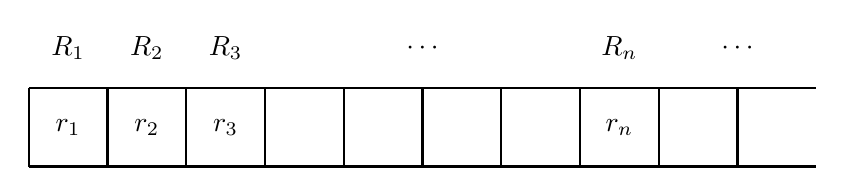
\begin{tikzpicture}
		\draw[thick] (0, 1) -- (10, 1);
		\draw[thick] (0, 0) -- (10, 0);
		\foreach \i in {0, 1, ..., 9}{
			\draw[thick] (\i, 0) -- (\i, 1);
		}
		\foreach \i in {1, 2, 3}{
			\node at (\i - 0.5, 1.5) {$R_{\i}$};
			\node at (\i - 0.5, 0.5) {$r_{\i}$};
		}
		\node at (5, 1.5) {$\cdots$};
		\node at (7.5, 1.5) {$R_{n}$};
		\node at (7.5, 0.5) {$r_{n}$};
		\node at (9, 1.5) {$\cdots$};
	\end{tikzpicture}
	\caption{Cinta y registros}
	\label{fig: cinta_y_registros}
\end{figure}

Ahora, las instrucciones que podemos utilizar se dividen en cuatro tipos:
\begin{enumerate}
	\item Cero: Para cada $n\in\omega^{+}$ la instrucción $Z\pa*{n}$ indica que se anota $0$ en el $n$-ésimo registro, es decir, en $R_{n}$ se instancia $r_{n}\gets 0$.
	\item Sucesor: Para cada $n\in\omega^{+}$ la instrucción $S\pa*{n}$ indica que se le suma $1$ al contenido del $n$-ésimo registro, es decir, en $R_{n}$ se instancia $r_{n}\gets r_{n} + 1$.
	\item Transferir: Para cada $n, m\in\omega^{+}$ la instrucción $T\pa*{n, m}$ indica que se transfiere el contenido del $n$-ésimo registro al $m$-ésimo registro sin modificar el contenido del $n$-ésimo registro, es decir, en $R_{m}$ se instancia $r_{m}\gets r_{n}$.
	\item Saltar: Para cada $n, m, k\in\omega^{+}$ la instrucción $J\pa*{n, m, k}$ indica que se compara el contenido de los registros $n$-ésimo y $m$-ésimo. Si sus contenidos son iguales, entonces se ejecuta la instrucción $k$; y si no, entonces se sigue con la siguiente instrucción.
\end{enumerate}

Una máquina URM es entonces una tupla de estas instrucciones, puesto que es importante conocer el orden en el cual se ejecutan las instrucciones.

Para entender mejor cómo se utilizan este tipo de máquinas, abordemos por ejemplo la ejecución de las instrucciones de la máquina $M =\pa*{J\pa*{2, 3, 5},S\pa*{1}, S\pa*{3},  J\pa*{1, 1, 1}}$ tomando como punto de partida la cinta que inicialmente se instancia con $r_{1} = 3$, $r_{2} = 2$ y $r_{n} = 0$ para cada $n > 2$. (Figura \ref{fig:cinta_inicial})

\begin{figure}[h!]
	\centering
	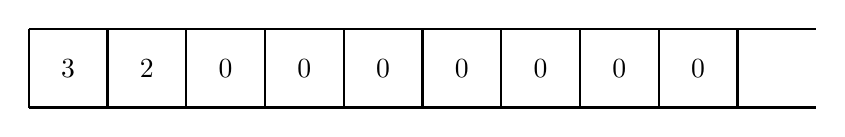
\begin{tikzpicture}
		\draw[thick] (0, 1) -- (10, 1);
		\draw[thick] (0, 0) -- (10, 0);
		\foreach \i in {0, 1, ..., 9}{
			\draw[thick] (\i, 0) -- (\i, 1);
		}
		\node at (0.5, 0.5) {3};
		\node at (1.5, 0.5) {2};
		\foreach \i in {2, 3,..., 8}{
			\node at (\i + 0.5, 0.5) {0};
		}
	\end{tikzpicture}
	\label{fig:cinta_inicial}
	\caption{Cinta inicial para la máquina $M$}
\end{figure}

La ejecución de la máquina $M$ se realiza yendo en secuencia por cada uno de los elementos de la tupla. Por lo tanto, se ejecuta primero la instrucción $J\pa*{2, 3, 5}$, la cual compara los contenidos de los registros $R_{2}$ y $R_{3}$. Puesto que $r_{2} = 2$ y $r_{3} = 0$, entonces no se satisface que $r_{2} = r_{3}$, por lo que se sigue con la siguiente instrucción. En esta iteración no se modificó ningún contenido de la cinta.

La siguiente instrucción en $M$ es $S\pa*{1}$. Entonces se suma $1$ al contenido en el primer registro, dando como resultado $r_{1} = 3 + 1 = 4$. En este caso sí se modificó el contenido de la cinta, y el resultado se puede ver en la figura \ref{fig:cinta_despues_de_s1}.

\begin{figure}[h!]
	\centering
	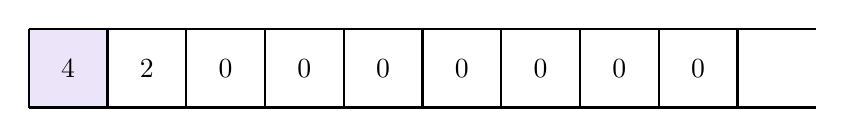
\begin{tikzpicture}
		\fill[violet!50!blue!10] (0, 0) rectangle (1, 1);
		\draw[thick] (0, 1) -- (10, 1);
		\draw[thick] (0, 0) -- (10, 0);
		\foreach \i in {0, 1, ..., 9}{
			\draw[thick] (\i, 0) -- (\i, 1);
		}
		\node at (0.5, 0.5) {4};
		\node at (1.5, 0.5) {2};
		\foreach \i in {2, 3,..., 8}{
			\node at (\i + 0.5, 0.5) {0};
		}
	\end{tikzpicture}
	\caption{Cinta después de ejecutar $S\pa*{1}$}
	\label{fig:cinta_despues_de_s1}
\end{figure}

Seguimos con la siguiente instrucción de la tupla que es $S\pa*{3}$, la cual indica que se debe sumar $1$ al tercer registro, dando $r_{3} = 0 + 1 = 1$, modificando la cinta como se ve en la figura \ref{fig:cinta_despues_de_s3}.

\begin{figure}[h!]
	\centering
	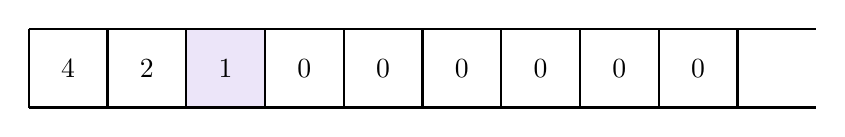
\begin{tikzpicture}
		\fill[violet!50!blue!10] (2, 0) rectangle (3, 1);
		\draw[thick] (0, 1) -- (10, 1);
		\draw[thick] (0, 0) -- (10, 0);
		\foreach \i in {0, 1, ..., 9}{
			\draw[thick] (\i, 0) -- (\i, 1);
		}
		\node at (0.5, 0.5) {4};
		\node at (1.5, 0.5) {2};
		\node at (2.5, 0.5) {1};
		\foreach \i in {3, 4,..., 8}{
			\node at (\i + 0.5, 0.5) {0};
		}
	\end{tikzpicture}
	\caption{Cinta después de ejecutar $S\pa*{3}$}
	\label{fig:cinta_despues_de_s3}
\end{figure}


La siguiente instrucción es $J\pa*{1, 1, 1}$ la cual pide comparar los contenidos del registro $1$. Puesto que trivialmente $r_{1} = r_{1}$, entonces debemos ejecutar después la instrucción $1$, es decir, debemos volver al inicio de la tupla $M$ y repetir el proceso de nuevo. En esta iteración no se modificó la cinta.

Ahora, al ejecutar $J\pa*{2, 3, 5}$ de nuevo se comparan los contenidos en los registros $r_{2}$ y $r_{3}$. Puesto que $r_{2} = 2\neq 1 = r_{3}$, entonces proseguimos con la siguiente instrucción. En esta iteración no se modificó tampoco la cinta.

Continuando con la instrucción $S\pa*{1}$, se suma $1$ al contenido en el primer registro, dando como resultado $r_{1} = 4 + 1 = 5$, el cual se puede ver en la figura \ref{fig:cinta_despues_de_s1_segunda_vez}.

\begin{figure}[h!]
	\centering
	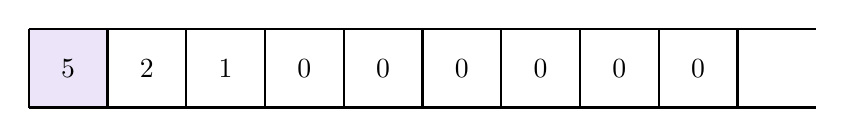
\begin{tikzpicture}
		\fill[violet!50!blue!10] (0, 0) rectangle (1, 1);
		\draw[thick] (0, 1) -- (10, 1);
		\draw[thick] (0, 0) -- (10, 0);
		\foreach \i in {0, 1, ..., 9}{
			\draw[thick] (\i, 0) -- (\i, 1);
		}
		\node at (0.5, 0.5) {5};
		\node at (1.5, 0.5) {2};
		\node at (2.5, 0.5) {1};
		\foreach \i in {3, 4,..., 8}{
			\node at (\i + 0.5, 0.5) {0};
		}
	\end{tikzpicture}
	\caption{Cinta después de ejecutar $S\pa*{1}$ por segunda vez}
	\label{fig:cinta_despues_de_s1_segunda_vez}
\end{figure}

Seguimos con la siguiente instrucción $S\pa*{3}$ obteniendo como resultado $r_{3} = 1 + 1 = 2$, modificando la cinta como se ve en la figura \ref{fig:cinta_despues_de_s3_segunda_vez}.

\begin{figure}[h!]
	\centering
	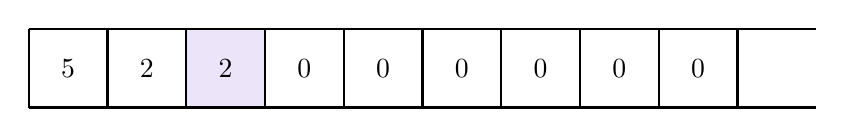
\begin{tikzpicture}
		\fill[violet!50!blue!10] (2, 0) rectangle (3, 1);
		\draw[thick] (0, 1) -- (10, 1);
		\draw[thick] (0, 0) -- (10, 0);
		\foreach \i in {0, 1, ..., 9}{
			\draw[thick] (\i, 0) -- (\i, 1);
		}
		\node at (0.5, 0.5) {5};
		\node at (1.5, 0.5) {2};
		\node at (2.5, 0.5) {2};
		\foreach \i in {3, 4,..., 8}{
			\node at (\i + 0.5, 0.5) {0};
		}
	\end{tikzpicture}
	\caption{Cinta después de ejecutar $S\pa*{3}$ por segunda vez}
	\label{fig:cinta_despues_de_s3_segunda_vez}
\end{figure}

La siguiente instrucción es $J\pa*{1, 1, 1}$. Puesto que trivialmente $r_{1} = r_{1}$, entonces se ejecuta la instrucción $1$, volviendo al inicio de la tupla $M$. En esta iteración no se modificó la cinta. Cuando se ejecuta $J\pa*{2, 3, 5}$, de nuevo se comparan los contenidos en los registros $r_{2}$ y $r_{3}$, y ya que $r_{2} = 2 = r_{3}$, entonces la siguiente instrucción a ejecutar es la número $5$.

Notemos que la tupla de instrucciones $M$ solamente tiene $4$ elementos, entonces no es posible realizar la instrucción $5$ que se pidió en $J\pa*{2, 3, 5}$. Cuando esto pasa, se interpreta que el algoritmo ha terminado al no haber más instrucciones a ejecutar. Por lo tanto, la salida de este algoritmo es la cinta $r_{1} = 5$, $r_{2} = r_{3} = 2$ y $r_{n} = 0$ para cada $n > 3$.

Por lo tanto, la ejecución completa de este algoritmo con la cinta de entrada $r_{1} = 3$, $r_{2} = 2$ y $r_{n} = 0$ para cada $n > 2$ es la que se muestra en la figura \ref{fig:ejecucion_completa_M}. En ella se puede ver cómo se van modificando los contenidos de los registros a medida que se ejecutan las instrucciones de la máquina $M$.

\begin{figure}[h!]
	\centering
	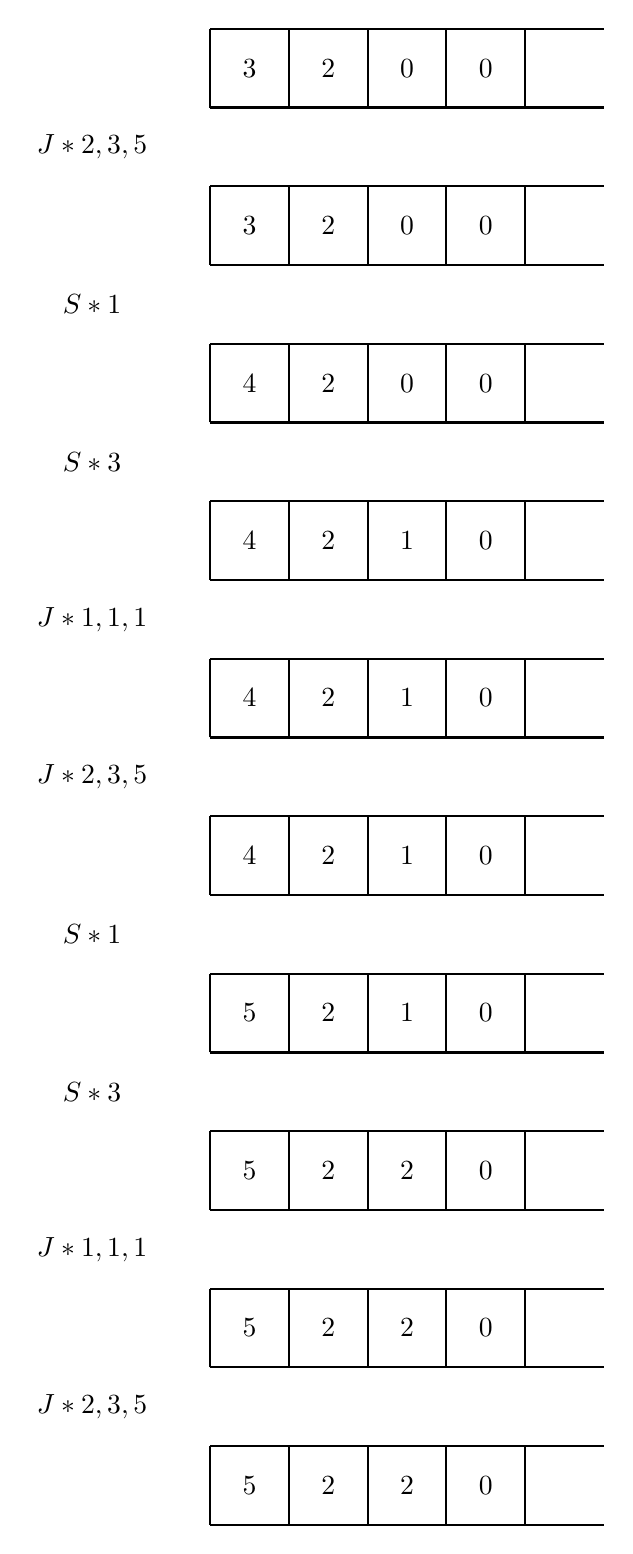
\begin{tikzpicture}
		\foreach \i in {1, 2,..., 10}{
			\draw[thick] (3, 17 - 2 *\i) -- (8, 17 - 2 * \i);
			\draw[thick] (3, 16 - 2 *\i) -- (8, 16 - 2 * \i);
			\foreach \j in {0, 1,..., 4}{
				\draw[thick] (3 +\j, 16 - 2 *\i) -- (3 +\j, 17 - 2 *\i);
			}
			\node at (6.5, 16.5 - 2 * \i) {0};
		}
		
		\foreach \i in {1, 2,..., 9}{
			\node at (5.5, 15.5 - 2 *\i) {$\ACABA$};
		}
		% primera
		\node at (3.5, 14.5) {3};
		\node at (4.5, 14.5) {2};
		\node at (5.5, 14.5) {0};
		% segunda
		\node at (1.5, 13.5) {$J\pa*{2, 3, 5}$};
		\node at (3.5, 12.5) {3};
		\node at (4.5, 12.5) {2};
		\node at (5.5, 12.5) {0};
		% tercera
		\node at (1.5, 11.5) {$S\pa*{1}$};
		\node at (3.5, 10.5) {4};
		\node at (4.5, 10.5) {2};
		\node at (5.5, 10.5) {0};
		% cuarta
		\node at (1.5, 9.5) {$S\pa*{3}$};
		\node at (3.5, 8.5) {4};
		\node at (4.5, 8.5) {2};
		\node at (5.5, 8.5) {1};
		% quinta
		\node at (1.5, 7.5) {$J\pa*{1, 1, 1}$};
		\node at (3.5, 6.5) {4};
		\node at (4.5, 6.5) {2};
		\node at (5.5, 6.5) {1};
		% sexta
		\node at (1.5, 5.5) {$J\pa*{2, 3, 5}$};
		\node at (3.5, 4.5) {4};
		\node at (4.5, 4.5) {2};
		\node at (5.5, 4.5) {1};
		% séptima
		\node at (1.5, 3.5) {$S\pa*{1}$};
		\node at (3.5, 2.5) {5};
		\node at (4.5, 2.5) {2};
		\node at (5.5, 2.5) {1};
		% octava
		\node at (1.5, 1.5) {$S\pa*{3}$};
		\node at (3.5, 0.5) {5};
		\node at (4.5, 0.5) {2};
		\node at (5.5, 0.5) {2};
		% novena
		\node at (1.5, -0.5) {$J\pa*{1, 1, 1}$};
		\node at (3.5, -1.5) {5};
		\node at (4.5, -1.5) {2};
		\node at (5.5, -1.5) {2};
		% decima
		\node at (1.5, -2.5) {$J\pa*{2, 3, 5}$};
		\node at (3.5, -3.5) {5};
		\node at (4.5, -3.5) {2};
		\node at (5.5, -3.5) {2};
	\end{tikzpicture}
	\caption{Ejecución completa de la máquina $M$}
	\label{fig:ejecucion_completa_M}
\end{figure}

Este ejemplo nos permite entender cómo es la lógica de este tipo de objetos. Cada una de las cintas que se obtienen a lo largo de la ejecución del algoritmo puede verse como una sucesión de números naturales. Por ejemplo, la cinta de entrada del ejemplo se formaliza como la sucesión $\pa*{3, 2, 0, 0, 0,\dotsc}$. Luego, para cada iteración $k$ del algoritmo se define la función $f_{k}:\omega\to\omega$ como la sucesión de números naturales que contienen los registros de la cinta en esa iteración, de modo que para cada $n\in\omega^{+}$, $f_{k}(n) = r_{n}$. De esta manera la ejecución del algoritmo dado por una máquina URM es una sucesión de funciones de números naturales $\pa*{f_{k}}_{k\in\omega}$ donde cada $f_{k}$ es la representación de los números de los registros de la cinta en la $k$-ésima iteración. Por convención la cinta de entrada del algoritmo se corresponde con la $0$-ésima iteración. Por lo tanto, como sucesiones, la ejecución de la máquina $M$ puede verse de la siguiente manera:
\[
	\begin{NiceArray}{ccccc}
		f_{0}\pa*{1} = 3 & f_{0}\pa*{2} = 2 & f_{0}\pa*{3} = 0 & f_{0}\pa*{4} = 0 &\cdots\\
		f_{1}\pa*{1} = 3 & f_{1}\pa*{2} = 2 & f_{1}\pa*{3} = 0 & f_{1}\pa*{4} = 0 &\cdots\\
		f_{2}\pa*{1} = 4 & f_{2}\pa*{2} = 2 & f_{2}\pa*{3} = 0 & f_{2}\pa*{4} = 0 &\cdots\\
		f_{3}\pa*{1} = 4 & f_{3}\pa*{2} = 2 & f_{3}\pa*{3} = 1 & f_{3}\pa*{4} = 0 &\cdots\\
		f_{4}\pa*{1} = 4 & f_{4}\pa*{2} = 2 & f_{4}\pa*{3} = 1 & f_{4}\pa*{4} = 0 &\cdots\\
		f_{5}\pa*{1} = 4 & f_{5}\pa*{2} = 2 & f_{5}\pa*{3} = 1 & f_{5}\pa*{4} = 0 &\cdots\\
		f_{6}\pa*{1} = 5 & f_{6}\pa*{2} = 2 & f_{6}\pa*{3} = 1 & f_{6}\pa*{4} = 0 &\cdots\\
		f_{7}\pa*{1} = 5 & f_{7}\pa*{2} = 2 & f_{7}\pa*{3} = 2 & f_{7}\pa*{4} = 0 &\cdots\\
		f_{8}\pa*{1} = 5 & f_{8}\pa*{2} = 2 & f_{8}\pa*{3} = 2 & f_{8}\pa*{4} = 0 &\cdots\\
		f_{9}\pa*{1} = 5 & f_{9}\pa*{2} = 2 & f_{9}\pa*{3} = 2 & f_{9}\pa*{4} = 0 &\cdots\\
	\end{NiceArray}
\]

Recordemos que el paso de un estado de la cinta a otro está completamente determinado por las instrucciones que tenga la máquina URM. Entonces, para poder manipular de manera adecuada tales instrucciones, y para poder describir de manera más explícita la sucesión de funciones $\set*{f_{k}}_{k\in\omega}$, interpretamos a las instrucciones como tuplas de la siguiente forma:
\[
	\begin{NiceArray}{cccc}
		Z\pa*{n}\to (0, n) & S\pa*{n}\to (1, n) & T\pa*{n, m}\to (2, n, m) & J\pa*{n, m, k}\to (3, n, m, k)
	\end{NiceArray}
\]

En este sentido se define al conjunto de \emph{instrucciones} para las máquinas URM de la siguiente manera.

\begin{definition}[Instrucciones]
	Se define al \emph{conjunto de instrucciones} para las máquinas URM como el siguiente conjunto de tuplas:
	\begin{align*}
		\INSTRUCCIONES\coloneqq&\set*{(0, n)\in\omega^{2}: n\in\omega^{+}}\cup\set*{(1, n)\in\omega^{2}: n\in\omega^{+}}\\
		&\cup\set*{(2, n, m)\in\omega^{3}: n, m\in\omega^{+}}\cup\set*{(3, n, m, k)\in\omega^{4}: n, m, k\in\omega^{+}}
	\end{align*}
\end{definition}

Con ello se define ahora lo que es una máquina URM, entendida como una sucesión finita de instrucciones.

\begin{definition}[Máquinas URM]
	Una \emph{máquina URM} es una tupla no vacía $M\in\INSTRUCCIONES^{<\omega}$, es decir, es tal que existe $n\in\omega^{+}$ para el cual $M\in\INSTRUCCIONES^{n}$.
\end{definition}

Recordando el ejemplo, al principio teníamos una cinta de entrada, la cual es una sucesión de elementos en $\omega$, donde solo un número finito de ellos son diferentes de cero. Lo anterior es debido a que un algoritmo siempre se debe recibir como entrada un número finito de datos, lo cual podemos codificar como tal cinta con esos datos dispuestos a lo largo de ella. Entonces dar como entrada al algoritmo una tupla de datos $\pa*{x_{1},\dotsc, x_{k}}\in\omega^{k}$ para algún $k\in\omega^{+}$ corresponde a definir la función $f_{0}:\omega\to\omega$ tal que para cada $n\in\omega^{+}$:
\[
	f_{0}(n)\coloneqq\begin{cases}
		x_{n}, & n\leq k\\
		0, &\text{en otro caso}
	\end{cases}
\]

Este concepto de datos de entrada es lo que justifica el hecho de que la cinta sea infinita, pues esa propiedad nos permite ingresar como entrada a un algoritmo un conjunto de datos arbitrariamente grande, e incluso poder usar los registros sobrantes como unidades de memoria que permitan almacenar datos auxiliares necesarios para computar lo que necesitamos.

Notemos que a lo largo de la descripción de la sucesión $\set*{f_{k}}_{k\in\omega}$ no hemos descrito qué pasa con $f_{k}(0)$. La razón es porque se utiliza ese dato como auxiliar para poder determinar qué pasa entre cada iteración, almacenando el número de instrucción que se debe ejecutar de la máquina URM.

Con todo esto se define cómo es que se determina la sucesión de las cintas dadas por la ejecución de las instrucciones de la máquina URM.

\begin{definition}[Ejecución de una máquina URM]
	Sean $M =\pa*{I_{1},\dotsc, I_{u}}$ una máquina URM y $x =\pa*{x_{1},\dotsc, x_{n}}\in\omega^{n}$ una tupla de entrada para algunos $n, u\in\omega^{+}$. Se define la \emph{ejecución} de la máquina $M$ con entrada $x$ como la sucesión de funciones $\set*{f_{k}}_{k\in\omega}$ definidas de la siguiente manera:
	\begin{enumerate}
		\item Para cada $m\in\omega$:
		\[
			f_{0}\pa*{m} =\begin{cases}
				1, & m = 0\\
				x_{m}, & 1\leq m\leq n\\
				0, &\text{en otro caso}
			\end{cases}
		\]
		\item Para cada $k\in\omega$, si $f_{k}\pa*{0}\leq u$ y además:
		\begin{enumerate}
			\item $I_{f_{k}\pa*{0}} = \pa*{0, i}$ para algún $i\in\omega^{+}$, se tiene entonces que para cada $m\in\omega$:
			\[
				f_{k + 1}\pa*{m} =\begin{cases}
					f_{k}\pa*{0} + 1, & m = 0\\
					0, & m = i\\
					f_{k}\pa*{m}, &\text{en otro caso}
				\end{cases}
			\]
			\item $I_{f_{k}\pa*{0}} = (1, i)$ para algún $i\in\omega^{+}$, se tiene entonces que para cada $m\in\omega$:
			\[
				f_{k + 1}\pa*{m} =\begin{cases}
					f_{k}\pa*{m} + 1, & m\in\set*{0, i}\\
					f_{k}\pa*{m}, &\text{en otro caso}
				\end{cases}
			\]
			\item $I_{f_{k}\pa*{0}} = (2, i, j)$ para algunos $i, j\in\omega^{+}$, se tiene entonces que para cada $m\in\omega$:
			\[
			f_{k + 1}\pa*{m} =\begin{cases}
				f_{k}\pa*{0} + 1, & m = 0\\
				f_{k}\pa*{i}, & m = j\\
				f_{k}\pa*{m}, &\text{en otro caso}
			\end{cases}
			\]
			\item $I_{f_{k}\pa*{0}} = (3, i, j, p)$ para algunos $i, j, p\in\omega^{+}$, se tiene entonces que para cada $m\in\omega$:
			\[
			f_{k + 1}\pa*{m} =\begin{cases}
				p, & m = 0\text{ y } f_{k}\pa*{i} = f_{k}\pa*{j}\\
				f_{k}\pa*{0} + 1, & m = 0\text{ y } f_{k}\pa*{i}\neq f_{k}\pa*{j}\\
				f_{k}\pa*{m}, &\text{en otro caso}
			\end{cases}
			\]
		\end{enumerate}
		\item Para cada $k > 0$, si $f_{k}\pa*{0} > u$, entonces $f_{k + 1} = f_{k}$.
	\end{enumerate}
	
	Decimos que la máquina $M$ \emph{termina su ejecución} dada la entrada $x$ si existe $k\in\omega$ tal que $f_{k}\pa*{0} > u$.
\end{definition}

Así formalmente hemos descrito el procedimiento que se había realizado en el ejemplo. Con esto dicho se define qué significa que una función sea \emph{computable} desde este enfoque. De manera simple podemos definir el valor que produce un máquina URM, para cada entrada $x\in\omega^{n}$ con $n\in\omega^{+}$, como el contenido del primer registro si la ejecución acaba.

Por ejemplo, considerando el ejemplo que describimos anteriormente, las instrucciones generan un algoritmo tal que dada la entrada $\pa*{3, 2}$, al acabar su ejecución, devuelve el valor $5$ en su primer registro. Resulta de hecho que la máquina que describimos, para cada par de entrada $\pa*{x, y}\in\omega^{2}$ el algoritmo termina y el valor del primer registro es su suma $x + y$. Por lo tanto, tal máquina es una implementación algorítmica de la función suma.

Sin embargo, dada la misma máquina $M =\pa*{J\pa*{2, 3, 5}, S\pa*{1}, S\pa*{3}, J\pa*{1, 1, 1}}$ podemos darle de entrada ternas $\pa*{x, y, z}\in\omega^{3}$, generando como resultado una función $f:\omega^{3}\to\omega^{\DIVERGE}$ con un comportamiento diferente al de la suma. Consideremos por ejemplo la entrada $(1, 1, 2)$, entonces se obtiene la siguiente ejecución:
\[
	\begin{NiceArray}{rcc}
		&&(1, 1, 2, 0, 0,\dotsc)\\
		J\pa*{2, 3, 5}&\to&(1, 1, 2, 0, 0,\dotsc)\\
		S\pa*{1}&\to&(2, 1, 2, 0, 0,\dotsc)\\
		S\pa*{3}&\to&(2, 1, 3, 0, 0,\dotsc)\\
		J\pa*{1, 1, 1}&\to&(2, 1, 3, 0, 0,\dotsc)\\
		J\pa*{2, 3, 5}&\to&(2, 1, 3, 0, 0,\dotsc)\\
		S\pa*{1}&\to&(3, 1, 3, 0, 0,\dotsc)\\
		S\pa*{3}&\to&(3, 1, 4, 0, 0,\dotsc)\\
		J\pa*{1, 1, 1}&\to&(3, 1, 4, 0, 0,\dotsc)\\
		J\pa*{2, 3, 5}&\to&(3, 1, 4, 0, 0,\dotsc)\\
		S\pa*{1}&\to&(4, 1, 4, 0, 0,\dotsc)\\
		&&\vdots
	\end{NiceArray}
\]

Notemos que al seguir ejecutando las instrucciones el tercer registro siempre es mayor al valor del segundo registro, entonces la instrucción $J\pa*{2, 3, 5}$ nunca redirige a la instrucción $5$; por lo que la ejecución nunca termina. En este caso se tiene que $f\pa*{1, 1, 2}\DIVERGE$. Se puede verificar también que si $\pa*{x, y, z}\in\omega^{3}$ es tal que $y\geq z$, entonces $f\pa*{x, y, z} = x + y - z$; y si $y < z$, entonces $f\pa*{x, y, z}\DIVERGE$.

Con esto podemos apreciar que la misma máquina URM puede darnos diferentes funciones únicamente variando el número de datos de entrada. Por lo tanto, la aridad de la función es esencial para determinar su comportamiento al ser computada mediante una máquina URM. 

\begin{definition}[Funciones URM-computables]
	Para cada máquina URM $M\in\INSTRUCCIONES^{k}$ para algún $k\in\omega^{+}$ y cada $n\in\omega^{+}$ se define la \emph{función URM-computable} de $M$ con aridad $n$ como la función parcial $\PHI{M}[n]:\omega^{n}\to\omega^{\DIVERGE}$ tal que para cada $x\in\omega^{n}$ con ejecución $\set*{f_{m}^{(x)}}_{m\in\omega}$:
	\[
		\PHI{M}[n](x) =\begin{cases}
			f_{p}^{(x)}\pa*{1}, & \exists u\pa*{f_{u}^{(x)}(0) > k}\land\pa*{p =\min\set*{u: f_{u}^{(x)}(0) > k}}\\
			\DIVERGE, &\text{en otro caso}
		\end{cases}
	\]
	
	Una función parcial $f:\omega^{n}\to\omega^{\DIVERGE}$ para algún $n\in\omega^{+}$ se denomina \emph{URM-computable} si existe una máquina URM $M$ tal que $f =\PHI{M}[n]$.
	
	Definimos al conjunto $\URMCOMPUTABLE$ como el conjunto de las funciones parciales que son URM-computables.
\end{definition}

\begin{notation}
	Dada una máquina URM $M$, denotaremos por $\PHI{M}$ a la función URM-computable $\PHI{M}[1]$.
\end{notation}

Como mencionamos antes, el objetivo de esta sección será demostrar que ambos enfoques de la computabilidad son equivalentes, o más formalmente, demostrar que se tiene la igualdad de conjuntos $\PARCIAL =\URMCOMPUTABLE$. La contención más sencilla de demostrar es que toda función parcial-recursiva es URM-computable.

\begin{theorem}
	Toda función parcial-recursiva es URM-computable.
\end{theorem}

\begin{proof}
	Probemos por inducción sobre el conjunto de funciones parcial-recursivas. Mostremos primero que las funciones básicas son URM-computables. Sean $n, k\in\omega^{+}$ con $k\leq n$ y definamos las máquinas $M_{1} = \pa*{\pa*{0, 1}}$, $M_{2} =\pa*{\pa*{1, 1}}$ y $M_{3} =\pa*{\pa*{2, k, 1}}$, entonces se sigue directamente que $\CERO =\PHI{M_{1}}[n]$, $\SUCESOR =\PHI{M_{2}}$ y $\PROYECCION{n}{k} =\PHI{M_{3}}[n]$.
\end{proof}
\comment{Completar}{Falta completar la demostración que las funciones parcial-recursivas son URM-computables.}

\subsection{Codificación de listas}

Para poder demostrar que $\URMCOMPUTABLE\subseteq\PARCIAL$ debemos ayudarnos de una herramienta esencial que es la \emph{enumeración}, lo cual significa que a cada máquina podemos asignarle un único número natural para poder tratar como entradas de funciones parcial-recursivas a los algoritmos mismos. Para poder hacer eso debemos representar a su vez las tuplas de números naturales como números naturales por sí mismos. A esto se le denomina \emph{codificación}. Aunque existen varias formas de poder codificar tuplas o listas de naturales, la forma más simple es por medio del teorema fundamental de la aritmética. La idea es poder hacer una inyección entre las listas y los naturales tratando a cada elemento de la lista como potencias de productos de primos. Por ejemplo, si tenemos la tupla $\pa*{1, 2, 3}\in\omega^{\DIVERGE}3]$, entonces podemos mapearlo al número $2^{1}3^{2}5^{3}$. Lo importante de esto es que el teorema fundamental de la aritmética nos asegura que tal producto de primos es único, por lo que podríamos recuperar la lista únicamente factorizando el número que lo representa y viendo sus potencias. Sin embargo, un problema de esta codificación algo burda es cuando tenemos listas con ceros, como por ejemplo las listas $\pa*{1, 2, 0, 0}$ y $\pa*{1, 2}$. Notemos en este caso que ambas listas serían mapeadas al número $2^{1}3^{2}$ justamente porque existen ceros al final. Una forma para poder arreglar esto es sumar $1$ a cada exponente en el mapeo. Por ejemplo, dadas las listas anteriores, podríamos mapear $\pa*{1, 2, 0, 0}$ a $2^{1 + 1}3^{2 + 1}5^{0 + 1}7^{0 + 1}$ y mapear $\pa*{1, 2}$ a $2^{1 + 1}3^{2 + 1}$, donde aquí las listas ahora están mapeadas a diferentes números naturales. Esta forma de mapear listas ya asegura una inyección debido a que ya no tendríamos potencias nulas con listas con ceros como elementos.

\begin{theorem}
	La función $f:\omega^{<\omega}\to\omega$ tal que para cada $n\in\omega$ y $x =\pa*{x_{1},\dotsc, x_{n}}\in\omega^{n}$ y se define por:
	\[
		f(x) =\prod_{k = 1}^{n}p_{k}^{x_{k} + 1}
	\]
	donde $p_{k}$ es el $k$-ésimo número primo es una inyección.
\end{theorem}

\begin{proof}
	Sean $x, y\in\omega^{<\omega}$ tales que $f(x) = f(y)$, entonces mostremos que $x = y$. Sean $n, m, x_{1},\dotsc, x_{n}, y_{1},\dots, y_{m}\in\omega$ tales que $x =\pa*{x_{1},\dotsc, x_{n}}$ y $y =\pa*{y_{1},\dotsc, y_{m}}$, entonces se tiene que:
	\[
		f(x) =\prod_{k = 1}^{n}p_{k}^{x_{k} + 1}\ ;\ f(y) =\prod_{k = 1}^{m}p_{k}^{y_{k} + 1}
	\]
	Ya que $f(x) = f(y)$, por el teorema fundamental de la aritmética sabemos que $n = m$ y para cada $k\leq n$ se tiene que $p_{k}^{x_{k} + 1} = p_{k}^{y_{k} + 1}$, de lo cual se sigue que $x_{k} = y_{k}$. Por lo tanto, $x = y$.
\end{proof}

El objetivo ahora entonces es verificar que ciertas propiedades de esta codificación son primitivo-recursivas.

\begin{definition}[Codificación de listas]
	Para cada $n\in\omega^{+}$ se define la función de \emph{codificación} $f_{n}:\omega^{n}\to\omega$ tal que para cada $x =\pa*{x_{1},\dotsc, x_{n}}\in\omega^{n}$:
	\[
		f_{n}(x) =\prod_{k = 1}^{n}p_{k}^{x_{k} + 1}
	\]
	Para cada $n\in\omega^{+}$ y cada $x =\pa*{x_{1},\dotsc, x_{n}}\in\omega^{n}$ se denotará por $\inner*{x} =\inner*{x_{1},\dotsc, x_{n}}$ a $f_{n}(x)$.
\end{definition}

\begin{theorem}{}{}
	Las funciones de codificación son primitivo-recursivas.
\end{theorem}

\begin{proof}
	Denotemos por $f:\omega\to\omega$ a la función que devuelve el $(n + 1)$-ésimo número primo, entonces se sigue para cada $n\in\omega^{+}$ que para cada $x\in\omega^{n}$:
	\[
		\inner*{x} =\prod_{k < n}\pa*{f(k + 1)}^{\PROYECCION{n}{k + 1}(x)}
	\]
	Ya que $f$, la función proyección, la potencia, suma y producto acotado son primitivo-recursivas, se sigue que las funciones codificación son primitivo-recursivas.
\end{proof}

De esta forma podemos definir entonces al conjunto de \emph{códigos} o \emph{secuencias} de listas como el conjunto de números naturales que son código de una tupla. De manera auxiliar definiremos a $1$ como la codificación de la lista vacía.

\begin{definition}[Secuencias]
	Definimos al conjunto de \emph{secuencias} o \emph{códigos} como el siguiente subconjunto de $\omega$:
	\[
		\SECUENCIAS\coloneqq\set*{1}\cup\set*{\inner*{x}\in\omega: x\in\omega^{<\omega}}
	\]
\end{definition}

\begin{theorem}
	El conjunto de códigos $\SECUENCIAS$ es primitivo-recursivo.
\end{theorem}

\begin{proof}
	Denotemos por $P\subseteq\omega$ al conjunto de números primos y $D\subseteq\omega^{2}$ a la relación ``divide a''. Notemos que la forma de caracterizar los códigos es que son productos de potencias de números primos consecutivos, lo cual puede verse como el conjunto de números $n$ tales que si $p$ es primo y divide a $n$, entonces todo primo menor a $p$ también divide a $n$. Definamos entonces la fórmula:
	\[
		\varphi\pa*{n} =\pa*{n > 0\land\pa*{\forall p\leq n}\pa*{\pa*{p\in P\land (p, x)\in D}\to\pa*{\forall q\leq p}\pa*{q\in P\to (q, x)\in D}}}
	\]
	Se tiene entonces que $\SECUENCIAS =\set*{n\in\omega:\varphi\pa*{n}}$; para el caso de $1$ se satisface también que $\varphi\pa*{1}$ por vacuidad ya que ningún primo es menor o igual que $1$. Ya que $P$ y $D$ son primitivo-recursivas, por los teoremas \ref{coll: prim_rec_formulas} y \ref{coll: prim_rec_acotado} sabemos entonces que $\SECUENCIAS$ es primitivo-recursiva.
\end{proof}

Ahora definimos dos operaciones básicas para poder manipular las listas que usaremos demasiado.

\begin{definition}[Máxima potencia, acceso y longitud]
	Definimos las siguientes funciones:
	\begin{enumerate}
		\item la función \emph{máxima potencia} $\MAXPOTENCIA:\omega^{2}\to\omega$ definida como sigue para cada $x, y\in\omega$:
		\[
			\MAXPOTENCIA\pa*{x, y} =\begin{cases}
				\max\set*{n\in\omega: x^{n}\mid y}, & x > 1, y > 0\\
				0, &\text{en otro caso}
			\end{cases}
		\]
		\item para cada $k\in\omega^{+}$, la función \emph{acceso} al $(k + 1)$-ésimo elemento $f_{k}:\omega\to\omega$ definida como sigue para cada $e\in\omega$:
		\[
			f_{k}(e) =\begin{cases}
				x_{k}, &\exists n\pa*{\exists x_{0},\dotsc, x_{n - 1}\in\omega}\pa*{k < n\land e = \inner*{x_{0},\dotsc, x_{n - 1}}}\\
				0, &\text{en otro caso}
			\end{cases}
		\]
		Denotaremos por $e\bra*{k}$ a $f_{k}\pa*{e}$.
		\item la función \emph{longitud} $\LONGITUD:\omega\to\omega$ definida como sigue para cada $e\in\omega$:
		\[
			\LONGITUD\pa*{e} =\begin{cases}
				n, &\exists n\exists x\in\omega^{n}\pa*{e =\inner*{x}}\\
				0, &\text{en otro caso}
			\end{cases}
		\]
	\end{enumerate}
\end{definition}

\begin{theorem}
	Las funciones máxima potencia, acceso y longitud son primitivo-recursivas.
\end{theorem}
\begin{proof}
	Para la función máxima potencia, si $D\subseteq\omega^{2}$ es la relación ``divide a'', se tiene lo siguiente para cada par $x, y\in\omega$:
	\[
		\MAXPOTENCIA\pa*{x, y} =\CARACTERISTICA{>}(x, 1)\CARACTERISTICA{>}\pa*{y, 0}\pa*{\pa*{\mu n < y + 1}\pa*{\pa*{x^{n}, y}\notin D} - 1}
	\]
	donde la resta se entiende como la resta en $\omega$. Ya que $D$ es primitivo-recursiva, se sigue que $\MAXPOTENCIA$ es primitivo-recursiva.
	
	Ahora, sea $k\in\omega$, entonces para la función de acceso al $(k + 1)$-ésimo elemento, si denotamo por $f:\omega\to\omega$ a la función que devuelve el $(n + 1)$-ésimo número primo, se tiene lo siguiente para cada $e\in\omega$:
	\[
		e\bra*{k} =\CARACTERISTICA{\SECUENCIAS}(e)\pa*{\MAXPOTENCIA\pa*{f(k), e} - 1}
	\]
	
	Finalmente, para la función longitud se tiene para cada $e\in\omega$ que:
	\[
		\LONGITUD\pa*{e} =\CARACTERISTICA{\SECUENCIAS}\pa*{e}\pa*{\mu n < e + 1}\pa*{\pa*{f(n), e}\notin D}
	\]
\end{proof}

\subsection{Codificación de máquinas URM}


Con todo esto desarrollado ahora podemos codificar a números naturales las máquinas URM. Recordemos que definimos a las máquinas URM como una secuencia de instrucciones, y cada una de estas instrucciones es a su vez representada como una tupla. Con todo esto, a cada máquina URM podemos directamente traducirla como la codificación de tales listas. Por ejemplo, si tomamos la máquina URM que calculaba la suma tendríamos la secuencia de tuplas:
\[
	M =\pa*{\pa*{1, 1},\pa*{1, 3},\pa*{3, 2, 3, 5},\pa*{3, 1, 1, 1}}
\]

La primer tupla $\pa*{1, 1}$ se codificaría como $\inner*{1, 1} = 2^{1 + 1}3^{1 + 1} = 2^{2}3^{2} = 36$ por ejemplo. Las demás tuplas se codificarían de la siguiente forma:
\[
	\begin{NiceArray}{c}
		\pa*{1, 1}\to\inner*{1, 1} = 2^{2}3^{2}\\
		\pa*{1, 3}\to\inner*{1, 3} = 2^{2}3^{4}\\
		\pa*{3, 2, 3, 5}\to\inner*{3, 2, 3, 5} = 2^{4}3^{3}5^{4}7^{5}\\
		\pa*{3, 1, 1, 1}\to\inner*{3, 1, 1, 1} = 2^{4}3^{2}5^{2}7^{2}
	\end{NiceArray}
\]
Entonces podríamos codificar a $M$ de manera similar de la siguiente forma:
\begin{align*}
	e &=\inner*{\inner*{1, 1},\inner*{1, 3},\inner*{3, 2, 3, 5},\inner*{3, 1, 1, 1}}\\
	&= 2^{\inner*{1, 1} + 1}3^{\inner*{1, 3} + 1}5^{\inner*{3, 2, 3, 5} + 1}7^{\inner*{3, 1, 1, 1} + 1}\\
	&= 2^{2^{2}3^{2} + 1}3^{2^{2}3^{4} + 1}5^{2^{4}3^{3}5^{4}7^{5} + 1}7^{2^{4}3^{2}5^{2}7^{2} + 1}
\end{align*}

Aunque este número es gigantescamente grande y computacionalmente en la práctica sería muy difícil de calcular, teóricamente es posible, pero el punto principal aquí es que este número es único y con él podemos recuperar cuales son las instrucciones exactas de $M$ usando todas las herramientas que hemos desarrollado. Por ejemplo, con esta máquina se tendría lo siguiente:
\[
	\begin{NiceArray}{c}
		e\bra*{0} =\inner*{1, 1}\\
		e\bra*{1} =\inner*{1, 3}\\
		e\bra*{2} =\inner*{3, 2, 3, 5}\\
		e\bra*{3} =\inner*{3, 1, 1, 1}
	\end{NiceArray}
\]

y de igual forma se tendría entonces:
\[
	\begin{NiceArray}{cccc}
		e\bra*{0}\bra*{0} = 1 & e\bra*{1}\bra*{0} = 1 & e\bra*{2}\bra*{0} = 3 & e\bra*{3}\bra*{0} = 3\\
		e\bra*{0}\bra*{1} = 1 & e\bra*{1}\bra*{1} = 3 & e\bra*{2}\bra*{1} = 2 & e\bra*{3}\bra*{1} = 1\\
		& & e\bra*{2}\bra*{2} = 3 & e\bra*{3}\bra*{2} = 1\\
		& & e\bra*{2}\bra*{3} = 5 & e\bra*{3}\bra*{3} = 1\\
	\end{NiceArray}
\]

Luego pudimos recuperar cada instrucción por medio del acceso a la lista. Sin embargo, notemos que $e\bra*{0}$ corresponde a la \emph{primera} instrucción de la máquina URM. Para no andar recorriendo los índices cada vez, la codificación de la máquina $M$ iniciará en $0$ solo para que los accesos a la lista y las instrucciones de $M$ correspondan directamente. En el ejemplo que estábamos analizando se sigue que su código es el siguiente:
\[
	\inner*{0, \inner*{1, 1},\inner*{1, 3},\inner*{3, 2, 3, 5},\inner*{3, 1, 1, 1}}
\]
Se define entonces lo siguiente.
\begin{definition}[Codificación de instrucciones y máquinas URM]
	Se definen los siguientes conjuntos de codificaciones de instrucciones y máquinas URM
	
	\begin{align*}
		\INSTRUCCIONESCOD &\coloneqq\set*{\inner*{0, n}\in\omega: n\in\omega^{+}}\cup\set*{\inner*{1, n}\in\omega: n\in\omega^{+}}\\
		&\cup\set*{\inner*{2, n, m}\in\omega: n, m\in\omega^{+}}\cup\set*{\inner*{3, n, m, k}\in\omega: n, m, k\in\omega^{+}}
	\end{align*}
	
	\[
		\URMCODIGO\coloneqq\set*{\inner*{0, x_{1},\dotsc, x_{n}}\in\omega: n\in\omega^{+}, x_{1},\dotsc, x_{n}\in\INSTRUCCIONESCOD}
	\]
\end{definition}

\begin{theorem}
	Los conjuntos $\INSTRUCCIONESCOD$ y $\URMCODIGO$ son primitivos recursivos.
\end{theorem}
\begin{proof}
	Para demostrar que $\INSTRUCCIONESCOD$ es primitivo-recursivo solo es necesario demostrar que cada uno de los conjuntos que lo componen son primitivos recursivos. Definamos los conjuntos $A_{1} =\set*{\inner*{0, n}\in\omega: n\in\omega^{+}}$, $A_{2} =\set*{\inner*{1, n}\in\omega: n\in\omega^{+}}$, $A_{3} =\set*{\inner*{2, n, m}\in\omega: n, m\in\omega^{+}}$ y $A_{4} =\set*{\inner*{3, n, m, k}\in\omega: n, m, k\in\omega^{+}}$. Notemos lo siguiente:
	\[
		\begin{NiceArray}{c}
			e\in A_{1}\iff\pa*{e\in\SECUENCIAS\land\LONGITUD\pa*{e} = 2\land e\bra*{0} = 0}\\
			e\in A_{2}\iff\pa*{e\in\SECUENCIAS\land\LONGITUD\pa*{e} = 2\land e\bra*{0} = 1}\\
			e\in A_{3}\iff\pa*{e\in\SECUENCIAS\land\LONGITUD\pa*{e} = 3\land e\bra*{0} = 2}\\
			e\in A_{4}\iff\pa*{e\in\SECUENCIAS\land\LONGITUD\pa*{e} = 4\land e\bra*{0} = 3}
		\end{NiceArray}
	\]
	Ya que $\SECUENCIAS$, $\LONGITUD$ y la función de acceso son primitivo-recursivas, por el teorema \ref{coll: prim_rec_formulas} se sigue que $A_{1}$, $A_{2}$, $A_{3}$ y $A_{4}$ son primitivo-recursivas, y luego $\INSTRUCCIONESCOD = A_{1}\cup A_{2}\cup A_{3}\cup A_{4}$ es primitivo-recursiva.
	
	Para $\URMCODIGO$, un elemento está en él si y solo si es un código y cada elemento de la lista es elemento de $\INSTRUCCIONESCOD$. Ya que $\LONGITUD$ es primitivo-recursiva, se tiene lo siguiente:
	\begin{align*}
		e\in\URMCODIGO\iff&\left(e\in\SECUENCIAS\land\LONGITUD\pa*{e} > 1\land e\bra*{0} = 0\right. \\
		&\left. \land\forall k\pa*{\pa*{k <\LONGITUD\pa*{e}\land k > 0}\to e\bra*{k}\in\INSTRUCCIONESCOD}\right) 
	\end{align*}
	Puesto que ya sabemos que $\INSTRUCCIONESCOD$ es primitivo-recursiva, entonces por los teoremas \ref{coll: prim_rec_formulas} y \ref{coll: prim_rec_acotado} se sigue que $\URMCODIGO$ es primitivo-recursiva.
\end{proof}
\begin{lemma}
	\label{lemma: ek_menor_e}
	Para cada $e\in\SECUENCIAS$ y cada $k <\LONGITUD\pa*{e}$, se satisface que $e\bra*{k} < e$.
\end{lemma}
\begin{proof}
	Se sabe que para cada número natural $n\in\omega$ se satisface que $n < 2^{n}$, entonces para cada $e\in\SECUENCIAS$ y cada $k <\LONGITUD\pa*{e}$ se satisface lo siguiente:
	\[
		e\bra*{k} < 2^{e\bra*{k}}\leq p_{k}^{e\bra*{k} + 1}\leq e
	\]
\end{proof}
\begin{theorem}[Máximo]
	Definimos a la función \emph{máximo} $\operatorname{Max}:\omega\to\omega$ de la siguiente manera:
	\[
		\operatorname{Max}\pa*{e}\coloneqq\begin{cases}
			\max\set*{x_{1},\dotsc, x_{n}}, & e\in\SECUENCIAS, e =\inner*{x_{1},\dotsc, x_{n}}\\
			0, &\text{en otro caso}
		\end{cases}
	\]
	Entonces $\operatorname{Max}$ es primitivo-recursiva.
\end{theorem}
\begin{proof}
	Definimos como ayuda al conjunto $M_{e}\subseteq\omega$ de elementos máximos de la lista codificada por el número $e\in\omega$ de la siguiente forma:
	\[
		m\in M_{e}\iff\pa*{\exists n <\LONGITUD\pa*{e}}\pa*{e\bra*{n} = m\land\pa*{\forall k <\LONGITUD\pa*{e}}\pa*{e\bra*{k}\leq e\bra*{n}}}
	\]
	Esto en esencia nos dice que un elemento está en $M_{e}$ si y solo si es elemento de la lista codificada por $e$ y es el elemento más grande de la lista. Puesto que la lista codificada es finita, siempre tiene un único elemento máximo (considerando que no es vacía), es decir que $M_{e}$ es un singulete, que debido a los teoremas \ref{coll: prim_rec_formulas} y \ref{coll: prim_rec_acotado}, es primitivo-recursivo. De esta manera podemos recuperar tal elemento iterando sobre todos los números menores o iguales a $e$, por el teorema \ref{lemma: ek_menor_e}, verificando cuál de ellos es el único elemento de $M_{e}$, pues con la definición de $M_{e}$ siempre aseguramos que tal valor está en la lista.
	\[
		\operatorname{Max}\pa*{e} =\CARACTERISTICA{\SECUENCIAS}\pa*{e}\pa*{\sum_{k = 0}^{e}k\CARACTERISTICA{M_{e}}\pa*{k}}
	\]
	Puesto que $\SECUENCIAS$ y $M_{e}$ son primitivo-recursivas, entonces $\operatorname{Max}$ es primitivo-recursiva.
\end{proof}

Esta función es necesaria para poder demostrar que las funciones siguientes son primitivo-recursivas, pues nos serán de ayuda para poder codificar el proceso iterativo del algoritmo de una máquina URM.

\begin{theorem}
	Las siguientes funciones son primitivo-recursivas:
	\begin{enumerate}
		\item La función \emph{número de instrucciones} $\operatorname{NumInstr}:\omega\to\omega$ que devuelve el número de instrucciones de una máquina URM codificada.
		\item La función \emph{número máximo de registros} $\operatorname{MaxReg}:\omega\to\omega$ que devuelve el registro más grande utilizado por la máquina URM.
	\end{enumerate}
\end{theorem}
\begin{proof}
	Para la función número de instrucciones tenemos lo siguiente:
	\[
		\operatorname{NumInstr}\pa*{e} =\CARACTERISTICA{\URMCODIGO}\pa*{e}\pa*{\LONGITUD\pa*{e} - 1}
	\]
	Para la función del máximo de registros podemos ir recorriendo todos los elementos de la lista, que son elementos de $\INSTRUCCIONESCOD$, y dependiendo del tipo de instrucción obtener el registro máximo entre el actual y los anteriores. Podemos codificarlo de manera recursiva definiendo primero la función $g:\omega^{2}\to\omega$ como sigue para cada $x, e\in\omega$:
	\[
		g\pa*{e, x} =
		\begin{cases}
			\operatorname{Max}\pa*{\inner*{x, e\bra*{1}}}, & e\bra*{0}\leq 1\\
			\operatorname{Max}\pa*{\inner*{x, e\bra*{1}, e\bra*{2}}}, & e\bra*{0} > 1
		\end{cases}
	\]
	la cual es primitivo-recursiva. Por lo tanto, podemos definir la función $f:\omega^{2}\to\omega$ como sigue de manera recursiva para cada $e, n\in\omega$:
	\[
		\begin{NiceArray}{c}
			f\pa*{e, 0} = 0\\
			f\pa*{e, n + 1} = g\pa*{e\bra*{n + 1}, f\pa*{e, n}}
		\end{NiceArray}
	\]
	la cual es primitivo-recursiva. Luego se tiene que la función número máximo de registros es primitivo-recursiva ya que satisface que para cada $e\in\omega$:
	\[
		\operatorname{MaxReg}\pa*{e} = \CARACTERISTICA{\URMCODIGO}\pa*{e}f\pa*{e,\LONGITUD\pa*{e} - 1}
	\]
\end{proof}